%!TEX root = ../../secondYearReport.tex
\paragraph{Work package 2 progress}

\subparagraph{Shared control method in interaction with compliant environment}

At JSI we studied mutual learning of human and robot in case of interaction with a compliant environment. A novel method for shared control between human and robotic skill was developed to efficiently facilitate the robot skill synthesis for the desired interaction. If the robotic skill is incrementally formed (online) while the physical interaction task is performed/taught by the human demonstrator then the robot has the capacity to generate the control commands for the robotic body already during the learning stage. However, the human is simultaneously controlling the robot body in order to teach it how to perform the given interaction task. Therefore, there can be a conflict between the human commands and commands generated by the currently obtained robotic skill. To solve this issue, an additional method was developed that can delegate the control responsibility between the two acting agents (i.e. human and robotic skill) over the robot body in tasks involving interaction with compliant environment.

While shared control is a well-studied subject in case of pure teleoperation \cite{Niemeyer2008}, only few studies exist in human-in-the-loop robot teaching framework. One of our previous studies \cite{Peternel2013} focused on developing a shared control method for teaching humanoid robot of compliant whole-body interaction with unpredictable environment in online manner. The control was shared percentually between human and incrementally built robotic skill based on the average error between demonstrated actions and actions from the robotic skill over entire task space up until the current observation time. The disadvantage of this method is that the human cannot efficiently inspect the performance of the currently learnt robotic skill in specific subspace (or state region) of the interaction task. In addition, percentually shared responsibility between the two agent makes it hard for the human to determine who is responsible for a potentially bad performance of the task.

To solve the above-mentioned drawbacks we developed a new method, where the control between the two agents is shared based on the existence of local models in the specific subspace (or state region) of the task. If no local models within the robotic skill exist for a specific subspace, where the task is currently performed, then the control responsibility is given to the human so that he can perform the task through the robot body and at the same time teach it. If local models within the robotic skill exist for the subspace where the task is currently performed, then the control responsibility is given to the robotic skill so that the human can inspect its performance. In case the observed performance is unsatisfactory, the human can update the robotic skill in that specific region. The advantage of this approach is that the skill inspection/correction can be done online (during the demonstration stage) without the need to stop the setup, as opposed to offline robot learning where the skill can be inspected only after the demonstration stage, and if corrections are required the demonstration stage has to be repeated.

The control was shared between the human and robotic skill as \cite{Peternel2013}
\begin{equation}
y_{cmd} = C \cdot y_{demo} + (1-C) \cdot y_{robot} ,
\label{eq:delegation}
\end{equation}
where $y_{cmd}$ is a vector of commands sent to the robotic mechanism, $y_{demo}$ is a vector of commands given by the human demonstrator, $y_{robot}$ is a vector of commands produced by the current robotic skill and $0 \leq C \leq 1$ is a weight factor that determines the influence of each agent. Pure human control is achieved when $C = 1$, and pure machine control is achieved when $C = 0$.

The practical implementation of the proposed method was done based on Locally Weighted Regression (LWR)\cite{Schaal1998}. LWR is an online machine learning method that approximates the non-linear model of demonstrated skill with a subset of local linear models. Each local linear model is fitted with a receptive field within the state region that determines its domain. The receptive fields are usually realised by a Gaussian kernel functions so that the closer the current input value is to its centre the higher the activation is. In term, higher higher activation of receptive field means higher influence of the corresponding local model on the output prediction. The prediction of output variable $y$ based on some new input variable $x$ is defined by a sum of contribution of all local models, where the models closer to the input variable have higher impact.

In the proposed shared control method the control responsibility between the two agents depends on the activation of the receptive fields of the local models of LWR. If the activation in a given state region is above some predefined threshold $w_{th}$, sufficient local models exist and therefore the control is given to the robotic skill ($C=0$) so that the human can inspect its performance. In opposite case, if activation is below $w_{th}$, no sufficient local models exist and therefore the control is given to the human ($C=1$) to perform an additional teaching. The method can be expressed as:
\begin{equation}
C = \begin{cases} 0 & \quad \text{if } w_{max} > (w_{th} + \frac{d}{2})
\\ \frac{ 1 + \cos \big(\pi \frac{w_{max} - (w_{th} - \frac{d}{2}) }{d}\big)}{2}  & \quad \text{if } (w_{th} - \frac{d}{2}) \leq w_{max} \leq (w_{th} + \frac{d}{2})
\\ 1 & \quad \text{if } w_{max} < w_{th} - \frac{d}{2}) \\ \end{cases}
\label{eq:factor}
\end{equation}
where $w_{max}$ is the activation of the model receptive fields \cite{Schaal1998} and $w_{th}$ is an activation threshold that we introduced to determine the model-proximity based shared control. The switching of responsibility between the human and robotic skill control is essentially binary to provide the human with a clear feedback about who is responsible for the given task performance. However, we implemented a cosine function to prevent sudden jumps between the two states of responsibility, were $d$ defines the width of switching function.

LWR allows incremental update of local models by feeding a new data point [$x$,$y$] each sample time. However, in such case it is hard for human to inspect the robotic skill performance of some subspace of the task as the skill is constantly changing/updating. Therefore we accumulated the training data points for some predefined amount of samples before we fed them to the LWR to update the models:
\begin{equation}
A_{new} = \begin{cases} A & \quad \text{if } C \neq 1
\\ [\thinspace A; \thinspace [x, \thinspace y]\thinspace ] & \quad \text{if } C = 1 \text{ and } length(A) < N_{acc}
\\ [\thinspace] & \quad \text{if } length(A) = N_{acc} \\ \end{cases}
\label{eq:accumulate}
\end{equation}
\begin{equation}
A_{in} = A(randperm(N_{acc}),\thinspace :)
\label{eq:shuffle}
\end{equation}
where $A$ is the training data accumulation buffer and the notation $A_{new}$ indicates that $A$ is updated at each iteration. $N_{acc}$ defines the accumulation length in samples before the new model update is made.  Before the data is fed to the LWR the training data in accumulation buffer randomly shuffled in $A_{in}$ buffer.

\begin{figure}[!t]
	\centering
	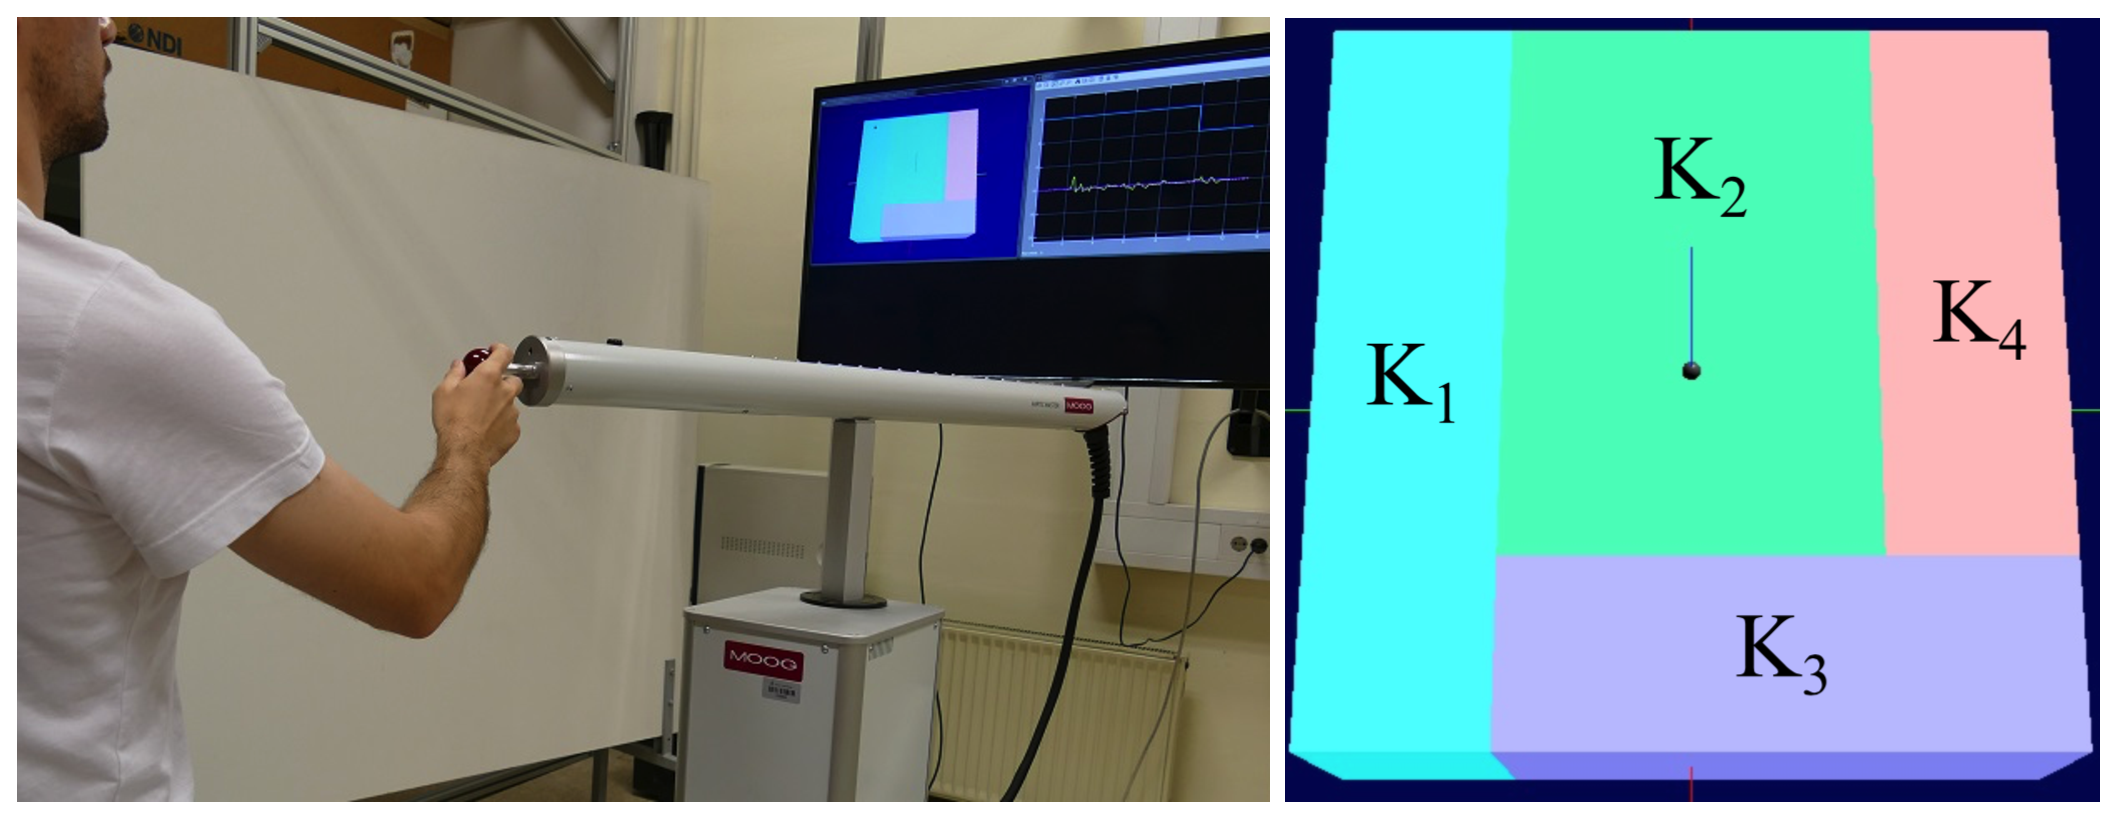
\includegraphics[width=0.99\textwidth]{setup.eps}
	\caption{Robot manipulator control interface consisting of HapticMaster robot and monitor for providing human with visual feedback (right photo). Compliant environment with different stiffness properties (left photo).}
	\label{fig:setup}
\end{figure}

\textbf{Experimental validation:} We validated the proposed method with the experiments on HapticMaster robot \cite{Linde2002}. The experimental setup is shown in Fig. \ref{fig:setup} left photo. The task of the robotic manipulator was to interact with a compliment environment in a way to produce some desired interaction force. The environment and robotic manipulator were simulated. We constructed a 0.4 by 0.4 m object so that its surface was in x-y (horizontal) plane of the reference frame, where different sections had different stiffness properties. See Fig. \ref{fig:setup} right photo for configuration of the object stiffness properties. The parameters were set $k_1=100$ N/m, $k_2=150$ N/m, $k_3=300$ N/m and $k_4=500$ N/m. The robotic manipulator had to produce a desired force $F_z=100$ N along z axis (vertical), which was perpendicular to the object surface. The necessary interaction force control policy was defined as:
\begin{equation}
F_{z} = K(x,y) \big(z_r-z_a\big),\label{en:robotimp}
\end{equation}
where $F_{z}$ is the interaction force acting between the manipulator and the object surface, $K(x,y)$ is the stiffness of the object in z axis, $z_a$ is actual and $z_r$ is reference position of the manipulator's end-effector in z axis. When the manipulator was on the softer section of the object surface (i.e. lower stiffness $K$), the reference position had to be put deeper inside the object to produce the desired force. In opposite case, when the manipulator was on the harder section of the object surface (i.e. higher stiffness $K$), the reference position had to be put closer to the surface to produce the same desired force.

The results of the experiment are shown in Fig. \ref{fig:models}. The top row shows the acquired models (robotic skill) for manipulator's displacement of reference position from the actual position in z axis. Each column represents the different stage of training data update. The time stamps of the update application are displayed on the top. The middle row shows the force prediction error of the obtained models at each stage. The bottom row shows the motion of the robot manipulator (thick black and green line) on the surface of the object (thin black rectangle). The black line shows the trajectory when the demonstrator had the control over the robotic manipulator's force production task. The green line shows the trajectory when robotic skill had the control over the robotic manipulator's force production task. The red crosses show the centres, while blue ellipses show the threshold activation ranges $w_{th}$ of the currently available local models that are part of robotic skill.

\begin{figure}[!t]
	\centering
	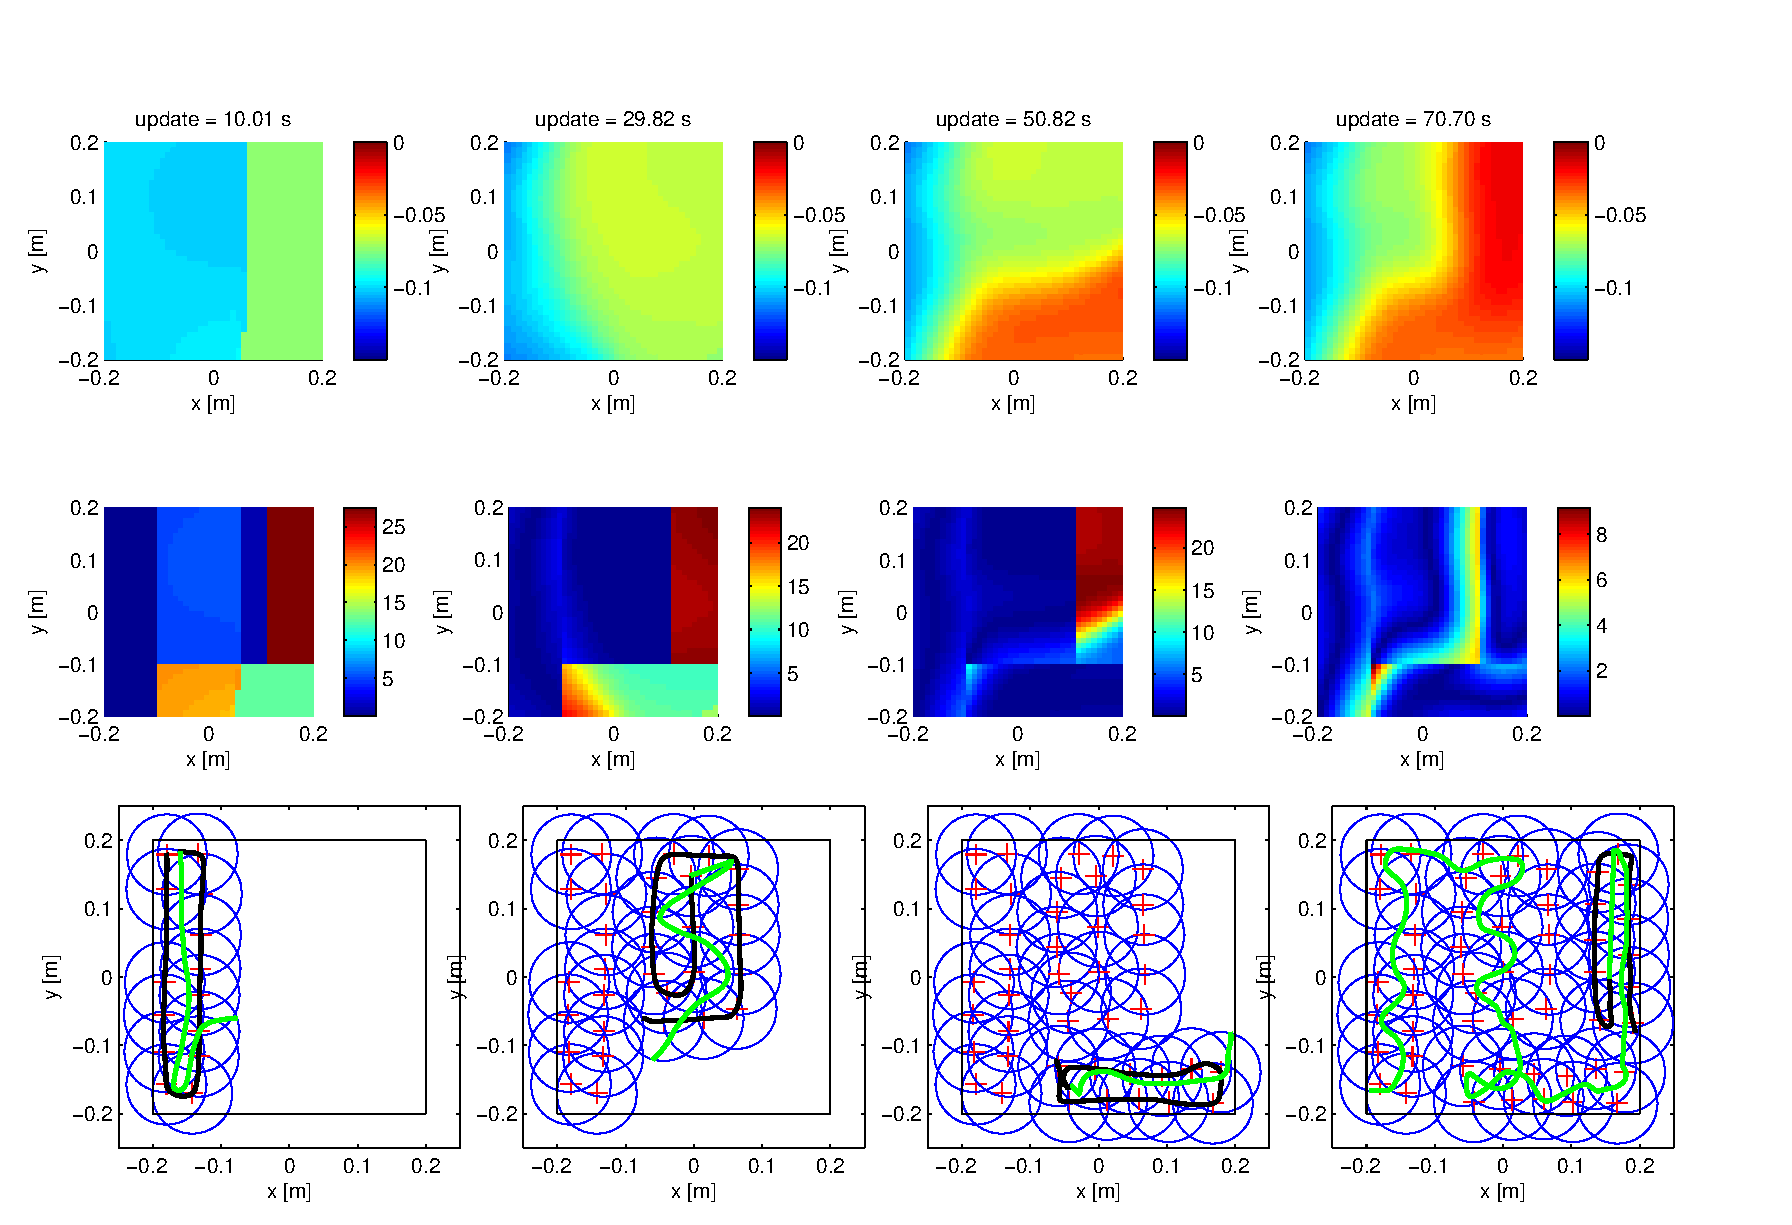
\includegraphics[width=0.99\textwidth]{models.eps}
	\caption{Result of the experiment. Graphs in each column correspond to the stage when robotic skill was updated. The upper row graphs show the performance of robotic skill in terms of control of reference position along z axis. The second row shows the error between the reference force and the force produced by the robotic skill. The third row shows the trajectory of motion of robotic manipulator end-effector when the control responsibility was given to human (black line) and when it was given to robot (green line). The influence of local models is shown by blue ellipses and its centres by red crosses.}
	\label{fig:models}
\end{figure}





\subparagraph{Human motor control learning during compliant interaction with environment}

\newcommand{\BF}{\mathbf{F}}
\newcommand{\BZ}{\mathbf{Z}}
\newcommand{\BA}{\mathbf{A}}
\newcommand{\BB}{\mathbf{B}}
\newcommand{\BC}{\mathbf{C}}
\newcommand{\BD}{\mathbf{D}}

In this study performed at UB we aimed to examine how humans learn compliant force dynamics and
modulate their whole-body motions to reach anticipated goals.  Here, we
present an experimental idea to measure the goal-directed movements against
compliant forces, and then illustrate the ongoing results which were conducted
for a few human subjects.  At this pilot stage, we are focusing on the simple
linear compliant case and discuss further experiments.  To deepen
understanding of the mechanism in humans, it would be beneficial to develop
the humanoid robot control in interacting with multiple compliant surfaces.

%%%%%%%%%%%%%%%%%%%%%%%%%%%%%%%%%%%%%%%%%%%%%%%%%%%%%%%%%%%%%%%%%%%%%%%%%%%%%%%%
%\section{Introduction}

\textbf{Introduction:}  Humans can learn how to control their own body movements in an uncertain
environment, and utilise it to predict the consequences of actions and to
achieve a behavioural goal \cite{Wolpert11, Davidson&Wolpert03}.  A
considerable amount of research has shown the human capabilities of
generalization in visuomotor learning and has been exploring the underlying
mechanisms \cite{Goodbody&Wolpert98, Krakauer06}.  A certain exposure to a new
physical environment facilitates to generalize the spatial and temporal
characteristics of the point-to-point movements via error-based learning and
perturbation paradigm. In the real-world interactions, there are varied and
complicated force dynamics (i.e., governed by not only simple linear
principles) when making a contact with an object and handling it. The optimal
functions seem to be perceptually learned via repetitive movements against the
force. However, to our knowledge, little is still known about how humans can
generalize the compliant force dynamics itself and utilize it to their future
motor plan.

The CoDyCo project has been investigating the whole-body coordination
mechanisms in arm reaching movements and the postural balance control in
assistive contact with rigid and/or compliant surfaces. Like humans, robots
are required to flexibly adjust their posture and to coordinate the physical
mobility with augmented autonomy. We expect that humans could generalize the
force principles in a cognitively robust way via force-feedback from the early
stage of the body movements. To explore the generalization mechanism of the
force dynamics in humans and to model it would provide a useful strategy in
humanoid robot control. The successful model could be exploited to effectively
control autonomous robots' whole-body balance in interacting with the
environment through supportive contacts.

In a pilot study, we focused on a simple case: linear compliant force. 
We employed a haptic device, Haptic Master (Moog, Inc.), which is controlled by 
a set of a computer programmes to render robotic manipulandum for force 
feedback. The pilot experiment measured the end-effector movements controlled 
by human subjects and analysed the dynamic properties of the movements against 
the compliant force and the performance.


%%%%%%%%%%%%%%%%%%%%%%%%%%%%%%%%%%%%%%%%%%%%%%%%%%%%%%%%%%%%%%%%%%%%%%%%%%%%%%%%
%\section{Methods}

%\subsection{Modelling}

\textbf{Modelling:} In general, spring-damper force ($\BF$) is formulated by the position and the
velocity with parameters: spring stiffness ($k$) and spring damping factor
($\lambda$).  Here, it is simplified for one direction ($\BZ$).
%
\begin{equation}
\BF = k \BZ^n + (\lambda \BZ^p) \dot{\BZ} \, .
\end{equation}
%

We employed the ready-made spring model in the Haptic API, where the 
compliant force formula was assigned to the device, the Haptic Master. 
The compliant force was rendered by the end-effector position and the 
velocity with the parameters in real-time (Fig. \ref{modelling}). 
%
\begin{figure}
	\centering
	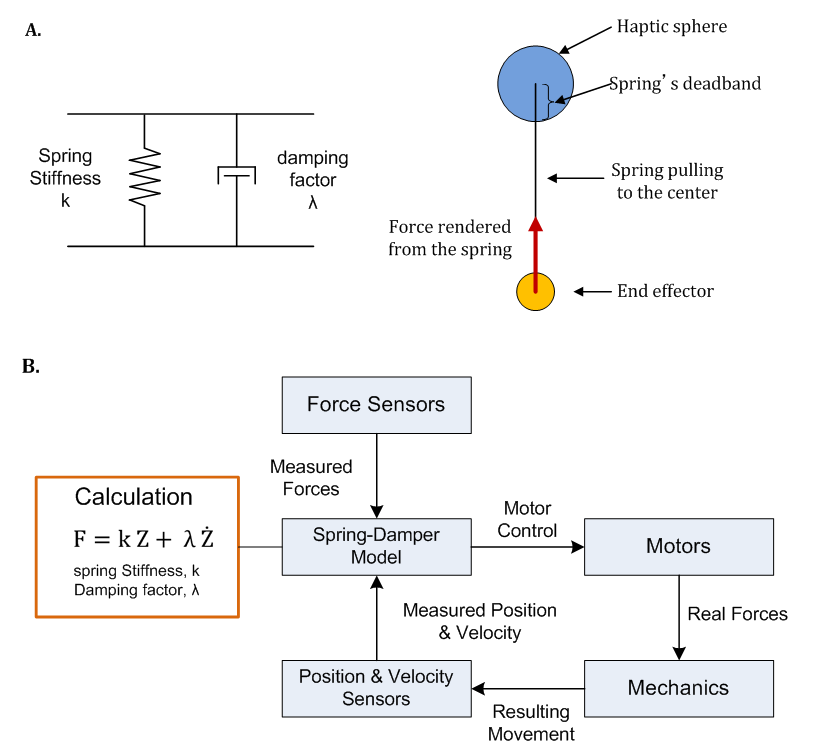
\includegraphics[scale=0.5]{fig1.png}
	\caption{A. The ready-made spring model in the Haptic API. B. Block 
		diagram of the compliant force control. The force is rendering
		based on the end-effector position and the velocity with parameters 
		(spring stiffness and damping factors) in the real time.}
	\label{modelling}
\end{figure}


%\subsection{Experimental Design}

\textbf{Experimental design:} As a pilot study, we employed a simple linear spring-damper formula:
%
\begin{equation}
\BF = k \BZ + \lambda \dot{\BZ} \, .
\end{equation}
%
The compliant force formula is assigned to the model in the Haptic
Master. Aiming to simplify analysing the performance, the forces and the
movements were constrained in the only one direction, here, in the vertical
(Z) direction to the ground.

Human subjects learned a spring compliant force via repetitive reaching
Bmovements to the first target (z = t1) in a certain period of time, - so
called ``Learning session''.  Then, they were asked to move the end-effector
to the second, or test, target (z = t2), which was set more far from the t1
position, as a test trial; so, more force would be required for this movement
(Fig. \ref*{design}). In order to achieve the t2 target, the participants would exploit
their prior knowledge of the force dynamics experienced via learning
session. We will evaluate whether and how the motion performance is likely to
follow the formula previously learned.
%
\begin{figure}
	\centering
	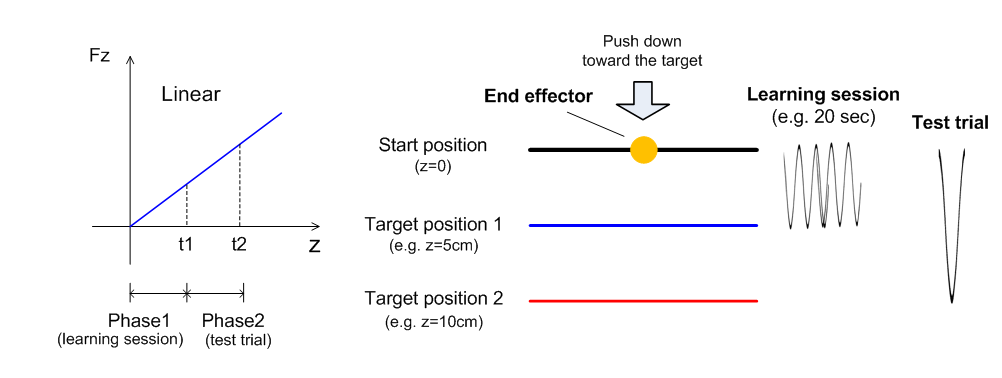
\includegraphics[scale=0.4]{fig2.png}
	\caption{Experimental Design. Two target positions were set: z = t1
		for learning session and z = t2 for test trial.}
	\label{design}
\end{figure}


%\subsection{Apparatus and Stimuli}

\textbf{Apparatus and Stimuli:} The haptic device, ``Haptic Master'' consisted of a large robotic rod with an
end-effector. The ``Home'' position, where was the centre of the end effector
is z = 0 at the workspace, was 110 cm from the ground. The spring position was
set at z = 0. In this study, the rod movements were restricted in the vertical
direction only.

The visual information about the task was provided at the computer display to
human subjects. The computer screen was located at the right side of the
Haptic Master from the subjects; where the centre of the screen was
approximately 80 cm from the centre of the robotic rod. The screen was
approximately 1 m away from the participants' standpoint, and 80 cm away from
the centre of the end effector position. The screen displayed the target
position and the end-effector position in real-time (Fig. \ref{stimuli}). The target
positions were set at z = t1 (50 mm for learning), and z = t2 (100 mm for
test).
%
\begin{figure}
	\centering
	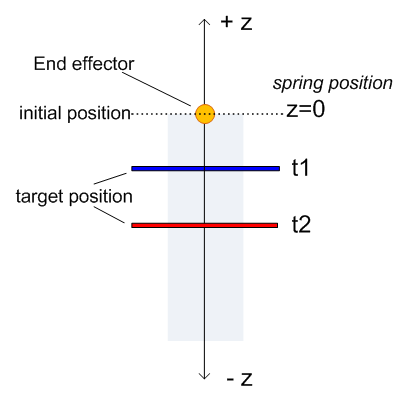
\includegraphics[scale=0.4]{fig3.png}
	\caption{Experimental visual stimuli. The end-effector and the two target 
		positions (z = t1 and z = t2) were visually indicated on the computer 
		screen.}
	\label{stimuli}
\end{figure}

%\subsection{Participants}

\textbf{Participants:} Six male subjects (age: 28.8 +/- 3.1 (SD), height: 175.3 cm +/- 7.1 (SD), 
weight: 79.5 kg +/- 17.8 (SD), one left-handed) voluntarily participated in the 
pilot experiment. All had normal or corrected to normal vision, and they had no 
known motor deficits and/or any limb injuries (self-reported). They were 
recruited from the student and staff population at University of Birmingham. 
(One was not naïve to the purpose of the experiment.)

%\subsection{Procedure and analyses}

\textbf{Procedure and analyses:} Participants stood in front of the haptic device and grasped the end-effector. 
Firstly, they conducted a practice session followed by the main blocks. They 
were required to make repetitive movements against compliant force generated by 
the device to learn the kinetic principle. The movements were monitored by 
visual information on the screen. Participants pushed the end-effector to reach 
the target position, and then released the end-effector to allow it to freely 
return to the initial position (z=0). They were asked to set the centre of the 
end-effector position on the target as accurate as possible. 

The main block consisted of two parts: Learning session and Test trial. In the 
Learning session, the target position was set at z= t1, described above. 
Participants controlled the end-effector by their own timing, or rhythm, per 
each movement in the current pilot study (the specific time windows were not 
set up by the programme for the series of movements: i.e., push the 
end-effector down from the start position and reach the target position). 
The visual feedback was given when the end-effector reached to the target; 
the target colour indicated this by changing from blue to yellow. 
Participants learnt the compliant force dynamics by the repetitive movements. 
he experimenter monitored the elapsed time using a stopwatch, and verbally 
informed the end of the session when 20 seconds passed. Participant stopped 
their repetitive movements immediately and prepared for the trial session. 

In the Test trial, participants moved the end-effector to the target (coloured 
red line, z = t2) three times based on the formula they previously learned. In 
this phase, no visual feedback in the relationship between the end-effector 
position and the target was given to the subjects.

One block consists of three sets (Learning session + Test trial). Participants 
conducted three blocks; so, 3 blocks in total, and 9 test trials. Under the 
current settings, the experiment was completed within approximately 20 minutes 
on average.

The dynamic properties of the point-to-point movements were measured: the
end-effector's position ($\BZ$), the velocity ($\dot{\BZ}$), and the force
($\BF_Z$) across the time. These were recorded by the 20 msec sampling rate
%and the
properties were analysed and compared between the linear and the non-linear
force conditions.

%%%%%%%%%%%%%%%%%%%%%%%%%%%%%%%%%%%%%%%%%%%%%%%%%%%%%%%%%%%%%%%%%%%%%%%%%%%%%%%%
%\section{Results and Discussions}




%\subsection{Ongoing Results}

\textbf{Results:} The end-effector position, velocity and force were recorded. Here, illustrates
the one participant's one block performance, as an example (Fig. \ref{results_1}).

In order to examine the each reaching movement, the data were extracted from 
the total between the start (z = 0.01m) and the end (approx. z = t2) positions, 
where the end-effector was released to return to the initial position. These 
points were determined by calculating the each inflection point (Fig. \ref{results_2}).

The data were averaged across three blocks; one block consisted of three
(Learning + Trial) sessions; so participants ideally completed 9 sessions in
total, but one (subj.03) accidentally completed only two blocks because of the
setting errors. The averaged numbers of repetitions were 152.8 +/- 45.6 (SD)
in the Learning session and 27.2 +/- 6.1 (SD) in the Test trial. All six
participants' averaged data (the end-effector position, velocity and force)
can be seen from Fig. \ref{results_3} to Fig. \ref{results_5}.
%
\begin{figure}
	\centering
	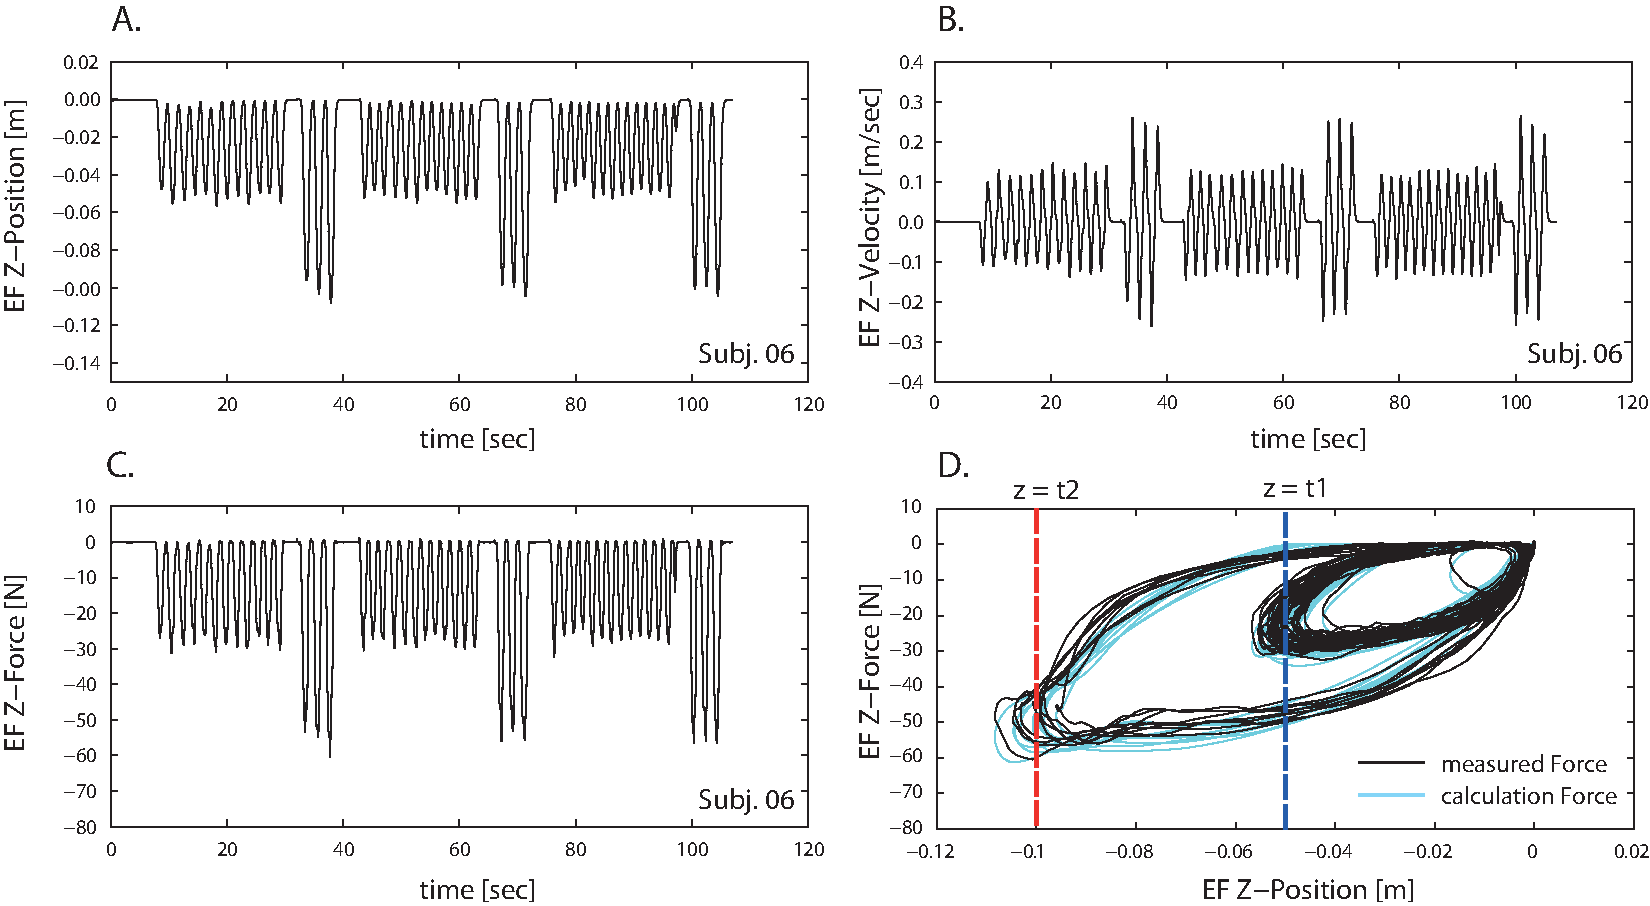
\includegraphics[scale=0.55]{fig4.pdf}
	\caption{The total recording of the completion of the first block.
		(Subj. 06). $\BA$. End-effector Z-position, $\BB$. Z-velocity and
		$\BC$. Z-force.  $\BD$. the relationship between the position and the
		force compared between the force directly measured by the sensor and the
		force calculated by the equation with the real time z-position and
		z-velocity.}
	\label{results_1}
\end{figure}
%
\begin{figure}
	\centering
	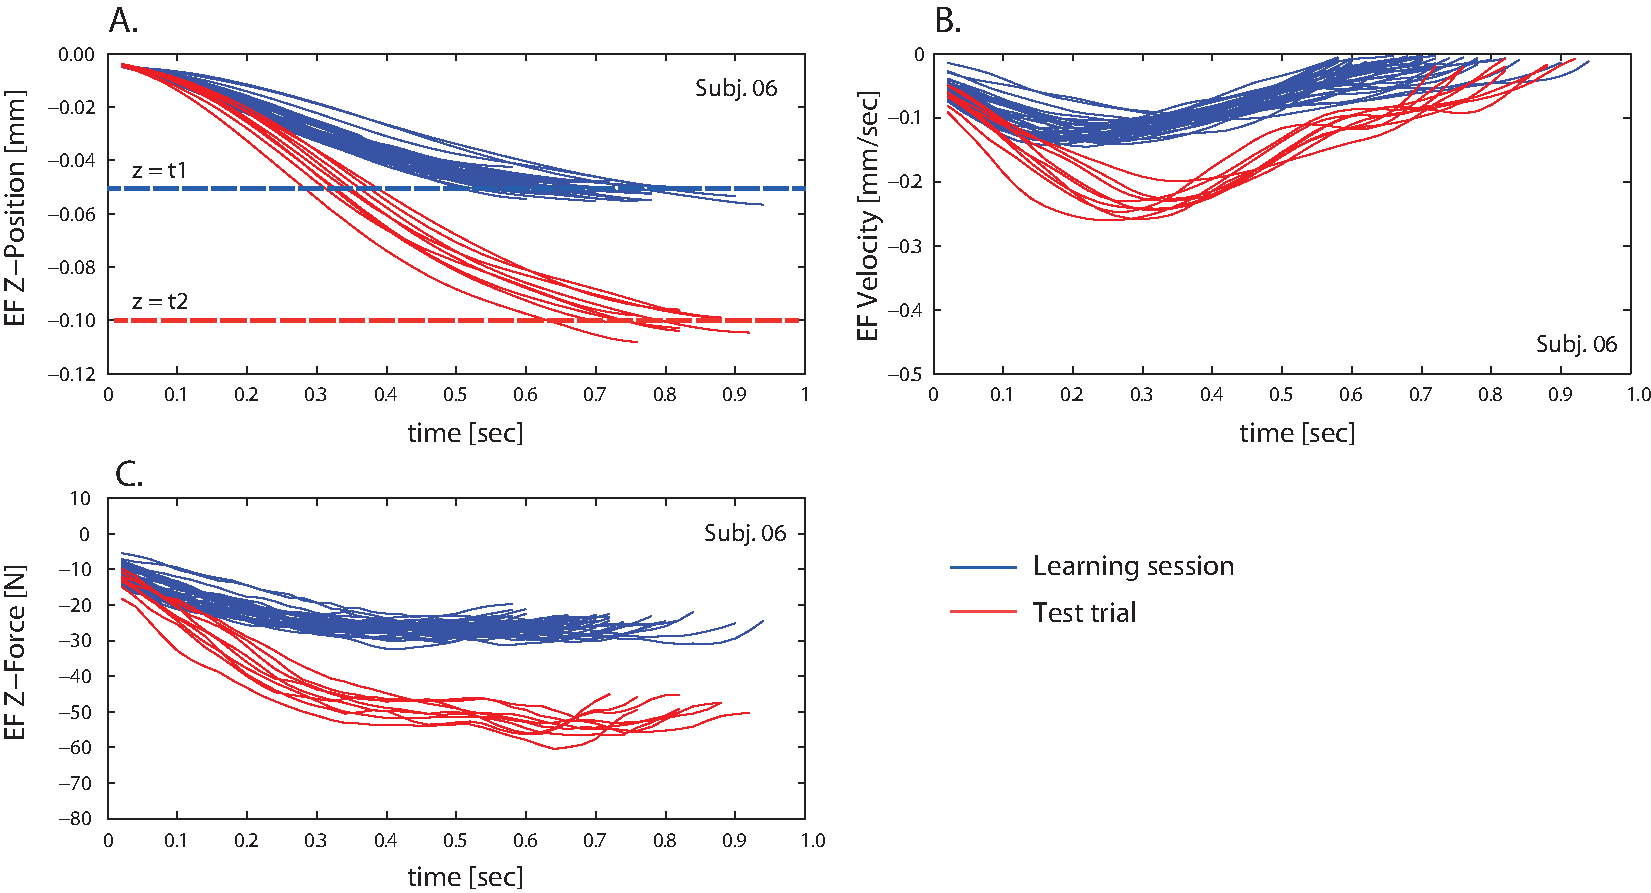
\includegraphics[scale=0.55]{fig5.pdf}
	\caption{Experimental data for one participant (the first block, three test 
		trials). Red lines represent the forces, which were directly measured by a 
		sensor at the end-effector. Blue lines represent the forces, which were 
		calculated in the real time by spring stiffness and damping factor with 
		the end-effector position.}
	\label{results_2}
\end{figure}
%
\begin{figure}
	\centering
	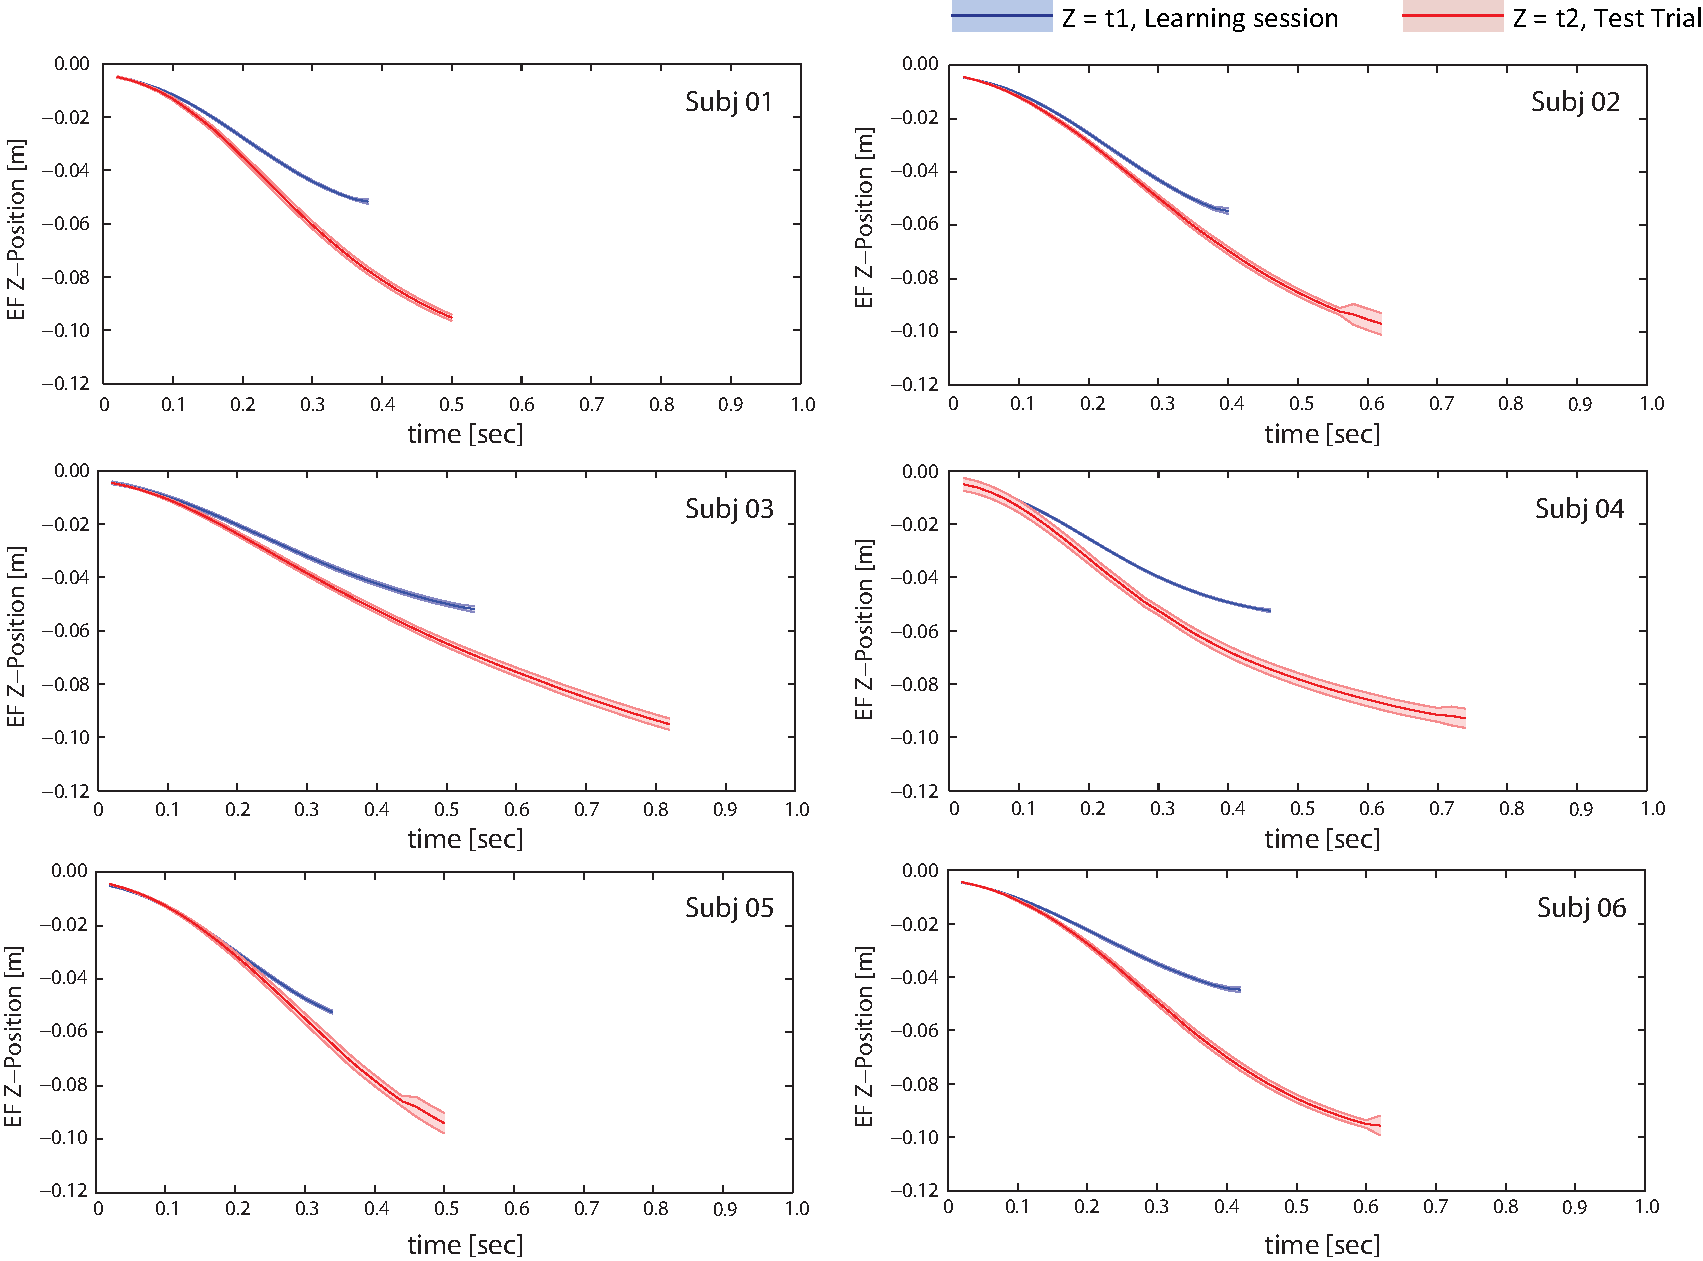
\includegraphics[scale=0.55]{fig6.pdf}
	\caption{The averaged end-effector z-position performance in the reaching 
		movements against the linear spring-damper force for 6 subjects. 
		The data were averaged across 3 blocks (9 (Learning + Trial) sessions). 
		The blue lines represent the average performance in the Learning session, 
		and the red in the Test trial, the coloured areas represent their standard 
		error respectively.}
	\label{results_3}
\end{figure}

\begin{figure}
	\centering
	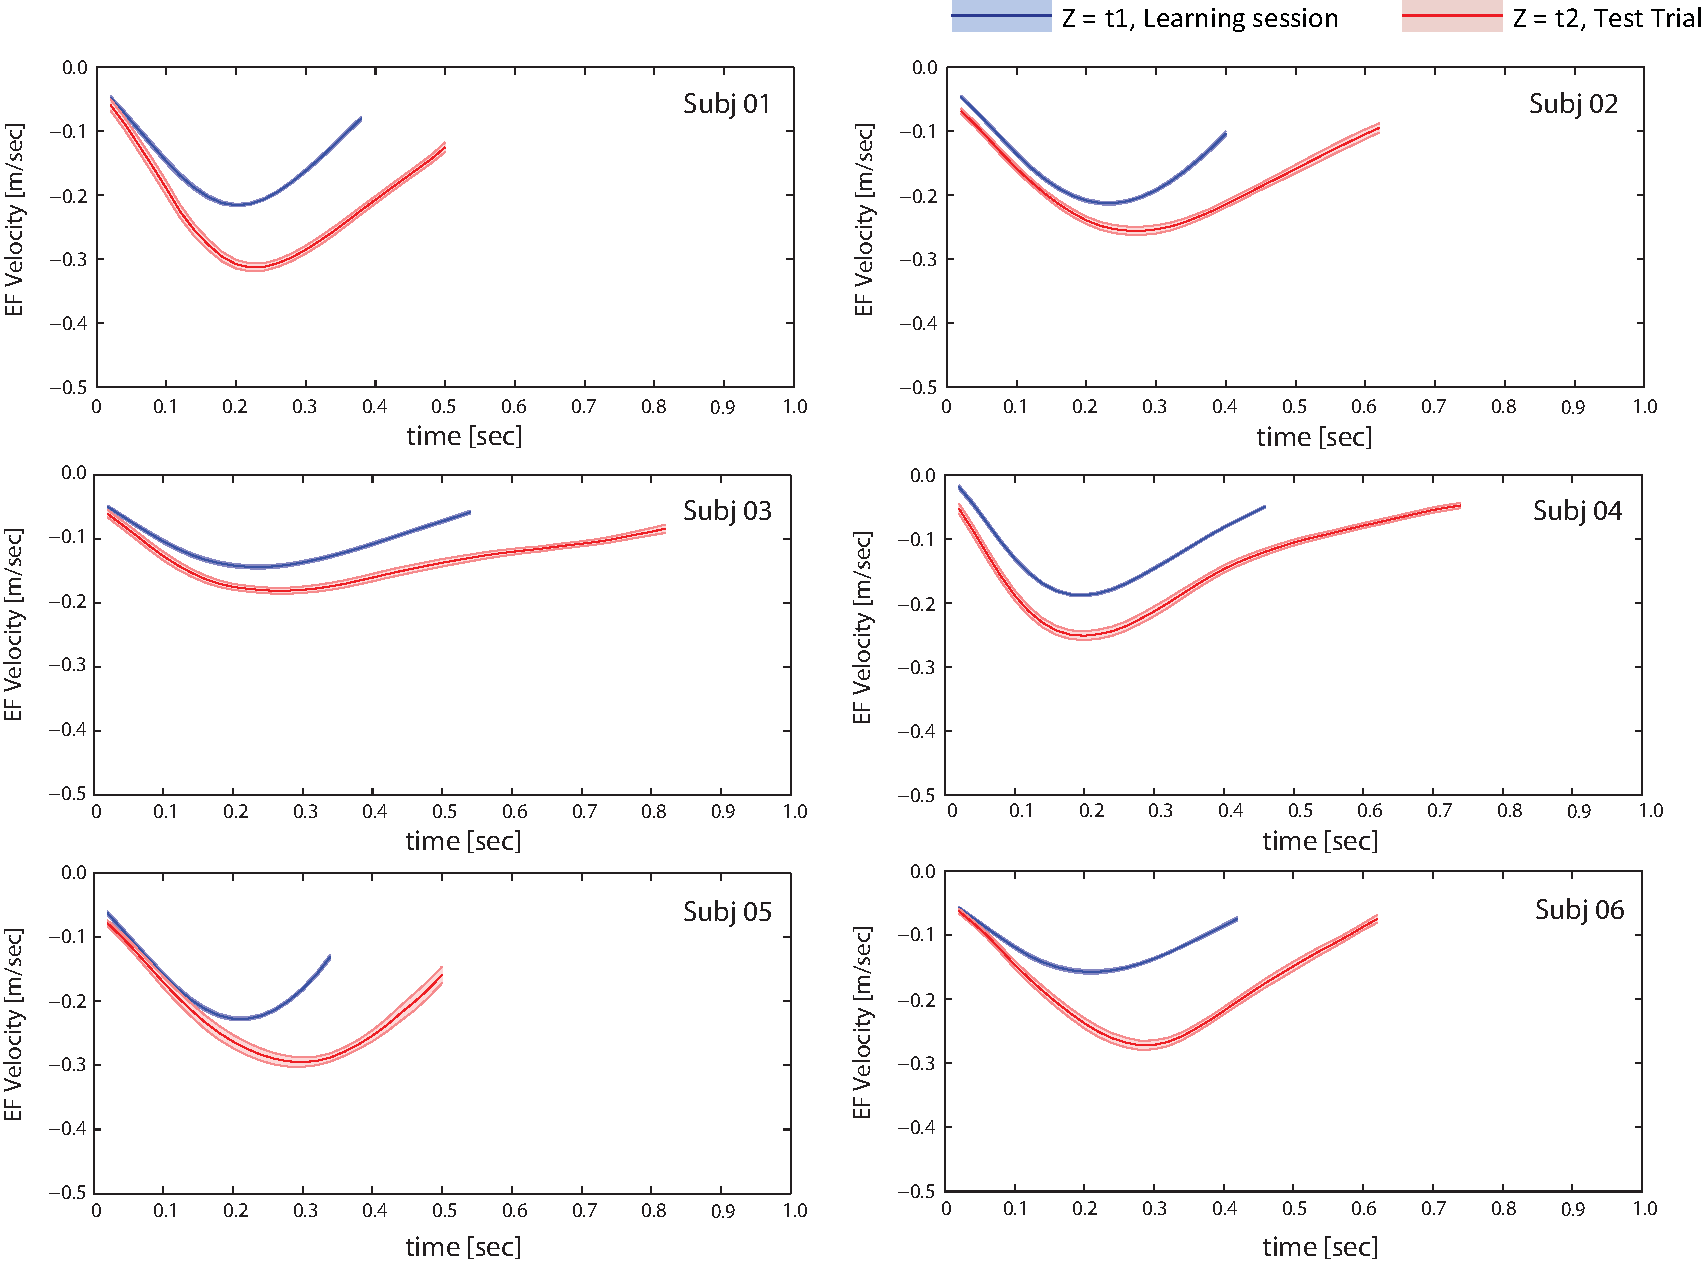
\includegraphics[scale=0.55]{fig7.pdf}
	\caption{The averaged end-effector z-velocity performance in the reaching 
		movements against the linear spring-damper force for 6 subjects. 
		The data were averaged across 3 blocks (9 (Learning + Trial) sessions). 
		The blue lines represent the average performance in the Learning session, 
		and the red in the Test trial, the coloured areas represent their standard 
		error respectively.}
	\label{results_4}
\end{figure}

\begin{figure}
	\centering
	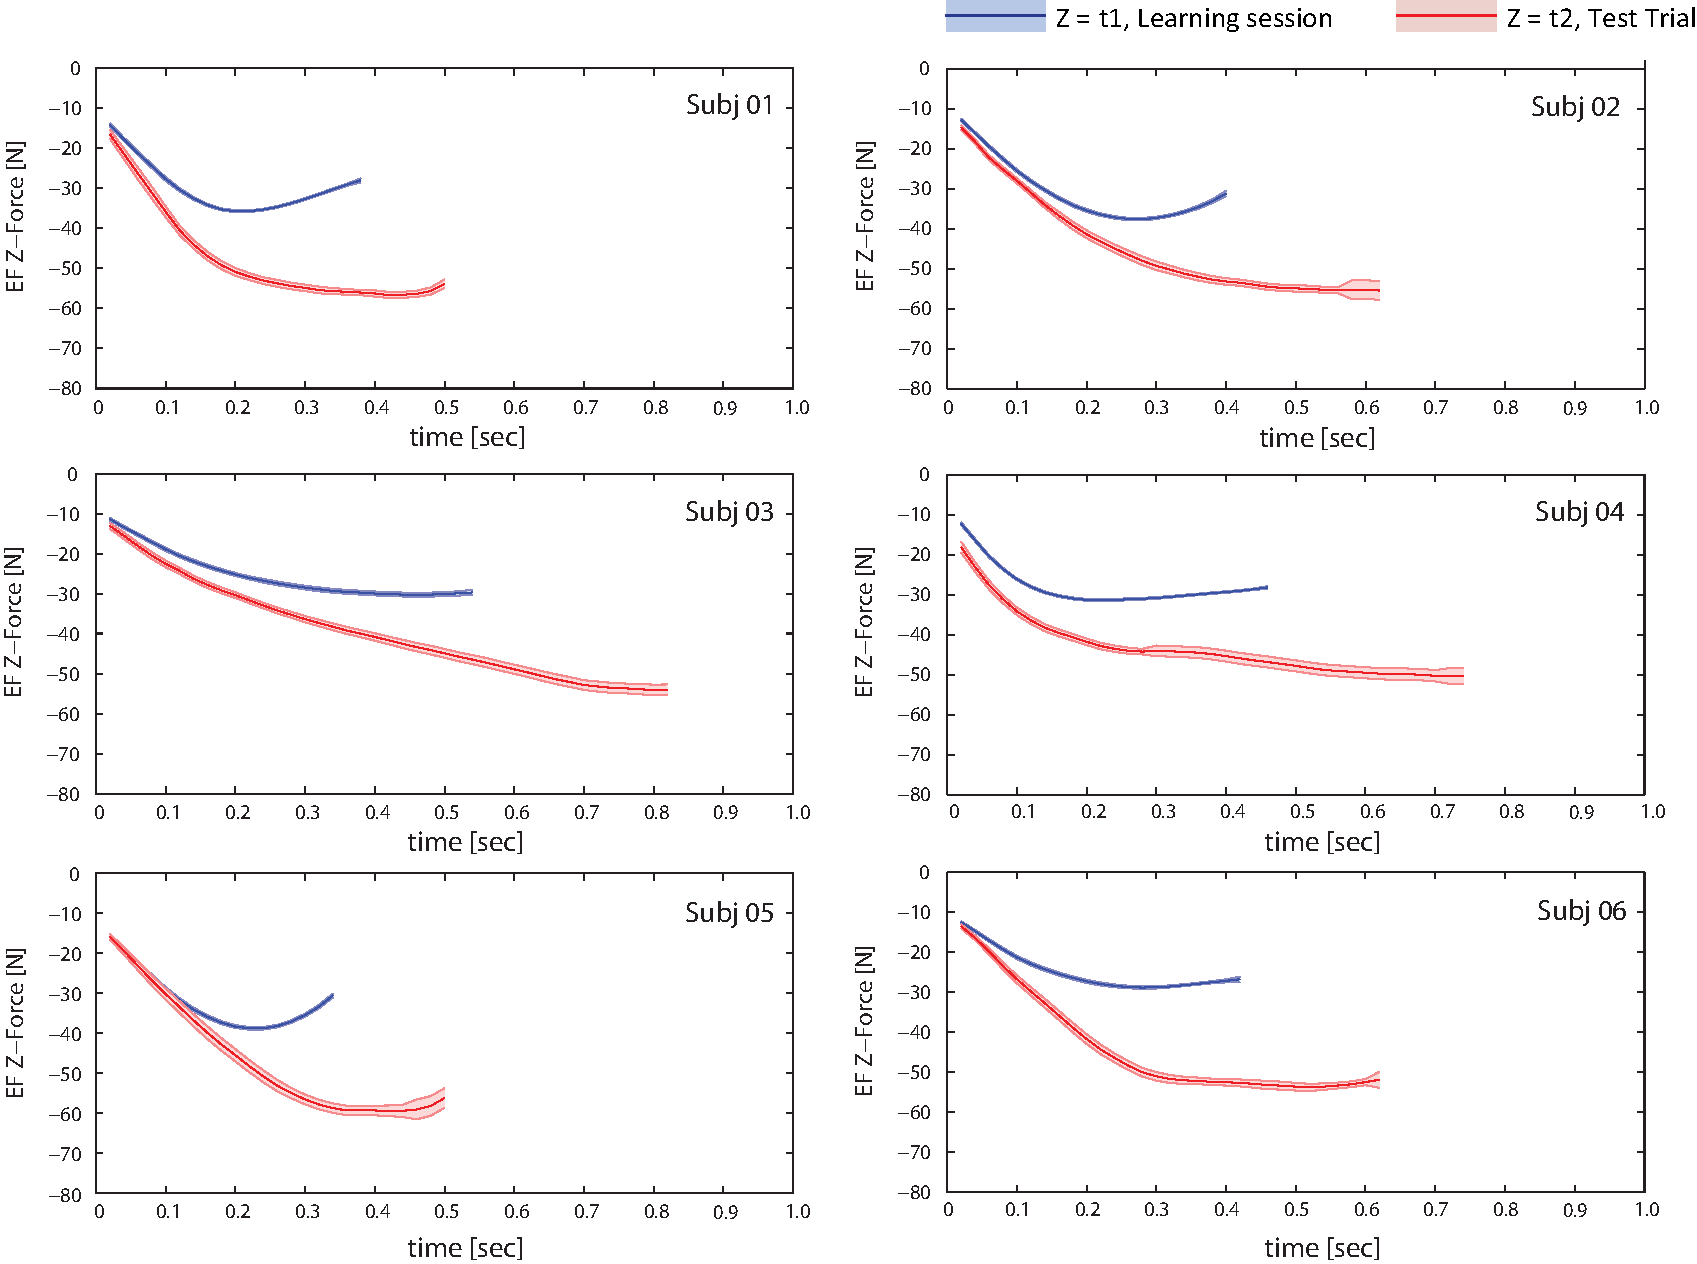
\includegraphics[scale=0.55]{fig8.pdf}
	\caption{The averaged end-effector z-force performance in the reaching 
		movements against the linear spring-damper force for 6 subjects. 
		The data were averaged across 3 blocks (9 (Learning + Trial) sessions). 
		The blue lines represent the average performance in the Learning session, 
		and the red in the Test trial, the coloured areas represent their standard 
		error respectively.}
	\label{results_5}
\end{figure}

\begin{figure}
	\centering
	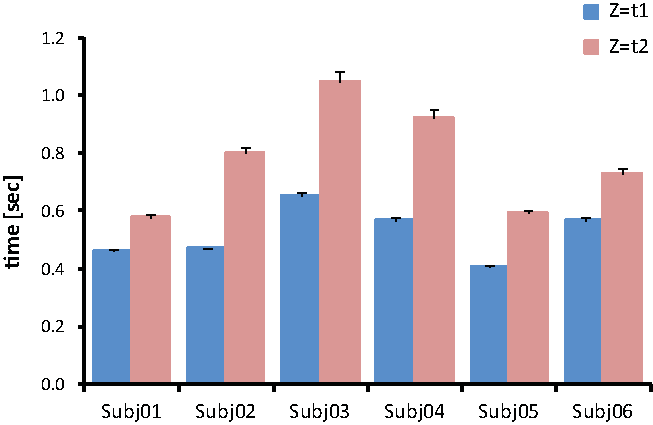
\includegraphics[scale=1]{fig9.pdf}
	\caption{Illustrate averaged time to reach the targets with the comparison 
		between the Learning session (blue) and the Test trial (red) for six 
		subjects. The error bars represents the standard error across the total 
		number of the repetitions.}
	\label{results_6}
\end{figure}


%\subsection{Brief Discussion}

\textbf{Discussion:} The \ref{results_6} showed that some participants (e.g., Subj.01, Subj.06) performed to 
reach the target position (z = t2) much faster than the expected time duration, 
which was estimated from the linear equation. That is, the t2 position was 
double distance of the t1 from the start position; so the reaching time would 
be estimated close to the double. The time would not be able to calculate by 
the simple linear calculation because the damping factor depends on the 
velocity, though.

This might be caused by the experimental design; that is, participants made
the repetitive movements with their own rhythms at the learning
session. Because they tend to keep their rhythms even in the consecutive trial
session, and then they might have unconsciously increased the force or
accelerated their speed to reach the target. This possibility can be seen at
their movement profiles (Fig. \ref{results_4}: velocity and Fig. \ref{results_5}: force). Several studies
have shown that time perception plays an important role in human motor control
\cite{Berret&Jean16, Rank&DiLuca15}; therefore, this timing issue should be
carefully considered into the experimental design and should avoid any
confounding factors. To do this, we will visually guide the participants'
movements with a certain time-windows in the future experiment.

Moreover, in the current pilot experiment, the judgment of reaching the target
was inaccurate. Although the participants received the visual feedback at the
learning session, it only indicated the end-effector crossed the target
position, and also there were no task reward. The inaccuracy would have
affected their force perception and movements \cite{Rank&DiLuca15} therefore,
in the next experiment, we will set a specific correct zone visually defined
by a more accurate way (e.g. the similar size of sphere of the end-effector)
as the target instead of the line indicators. The task completion in the
Learning session would be determined by their performance and individual
learning level would be evaluated by their correct movements.

The current analyses conducted for all performance in the test trial (reaching 
the target (z= t2) three times for each), but the performance might have needed 
to be evaluated focusing on the first trial only, because the first movement 
was directly affected by the learning session and the second and the third 
movements were gradually contaminated.

Overall, through the pilot experiment, we have learned the importance of the 
timing issue in interacting with compliant surface. We will improve the 
experimental design and strictly control the parameters (timing, speed, 
and the accuracy). 

In the future experiment, based on the linear case, we will measure the 
pattern under the non-linear compliant forces and examine the human 
goal-directed performance. Besides, as well as the spring-damper, it may 
help the understanding of the generalization if we employ another compliant 
force model (e.g. object surface).



\subparagraph{Experimental validation of CoM manipulability metric (Task 2.2 & Task 2.3)}

\newcommand{\BW}{\mathbf{W}}
\newcommand{\Bc}{\mathbf{c}}

After the introduction of a set of metrics to study, analyze and measure the ability to balance for both humans and legged robots we performed an experimental study to verify the application of the metrics for human postural control in contact with environment.  In the
experiments, the centers of mass of human subjects in different configurations were perturbed and joint torques were computed by inverse dynamics calculations.  We demonstrated that the metric is suitable for comparing different postures in the sense of the total required effort for the maintenance of balance.


\textbf{Human experiments:} To verify the application of the \textit{change-of-velocity---unit joint 
	impulse} ellipsoid for human studies, we performed experiments on human
subjects.  As already mentioned, this ellipsoid can be used to measure torque
efficiency in balancing motions.  So, in the experiments, we perturb the CoM
of the subjects (by a cable-pulley mechanism) in different configurations and
measure the contact forces/moments with force/torque sensors (see
Fig.~\ref{experimentsetup}).  Then we calculate the average total torque that
is done by the subjects at each configuration and compare them with the
results of manipulability analysis.  These steps are described in the
following subsections.

\begin{figure}
	\centering
	\begin{tabular}{c}
		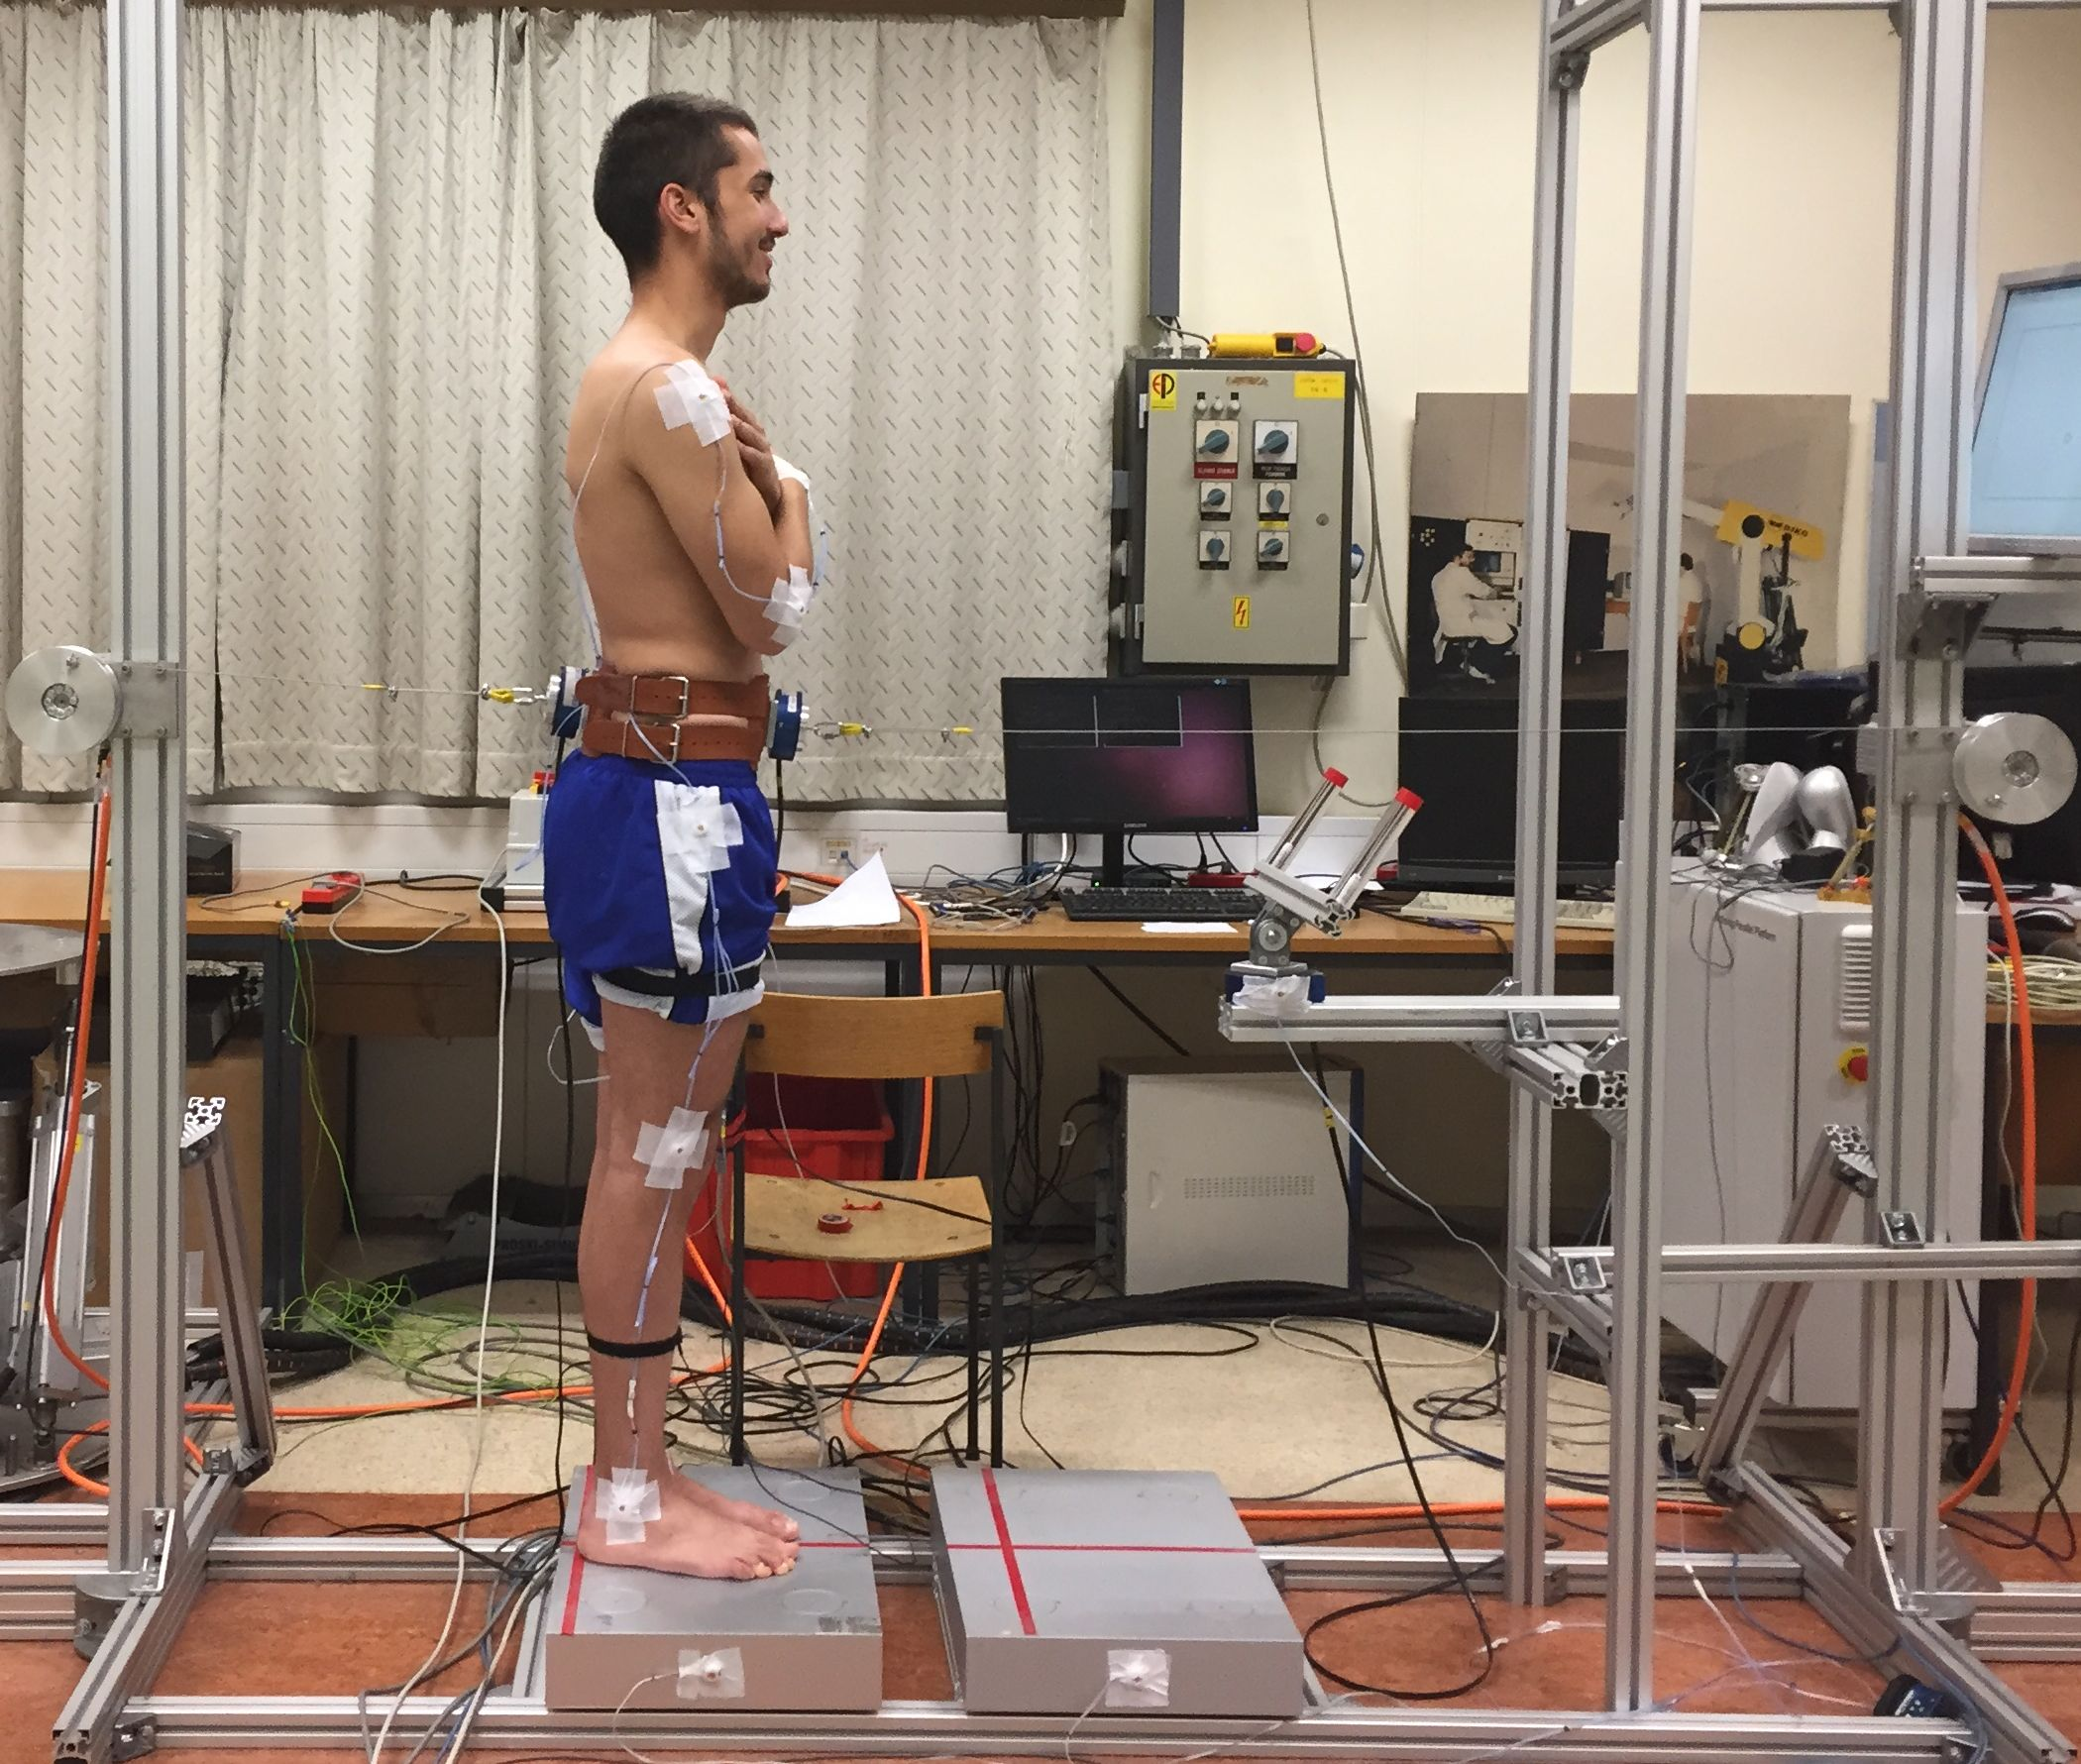
\includegraphics[width=0.75\columnwidth]{stance.jpg} \\
		(a)\\
		
	\end{tabular}
	\centering
	\begin{tabular}{cccc}
		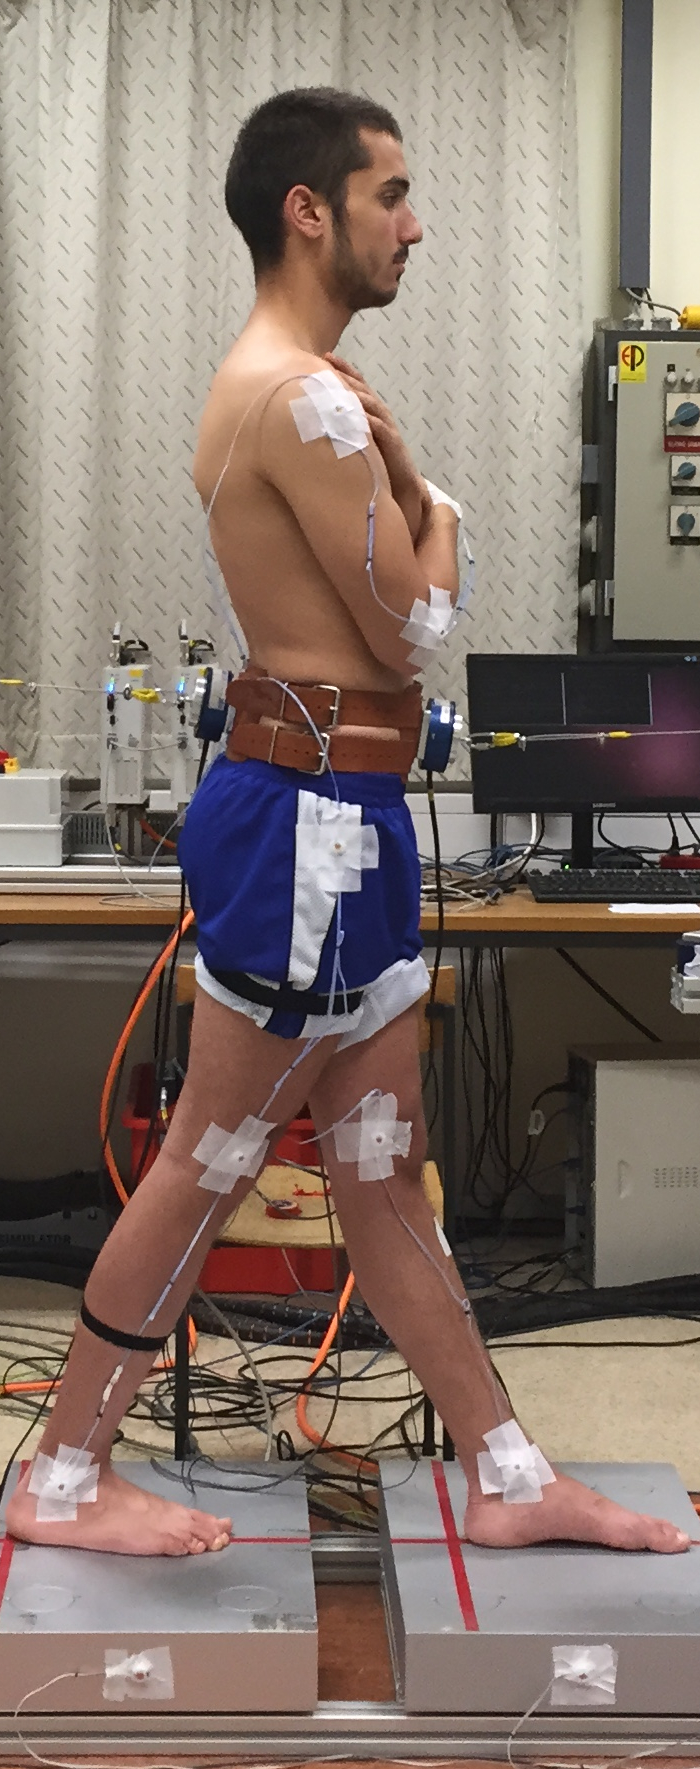
\includegraphics[width=0.2\columnwidth]{widestance.jpg} &
		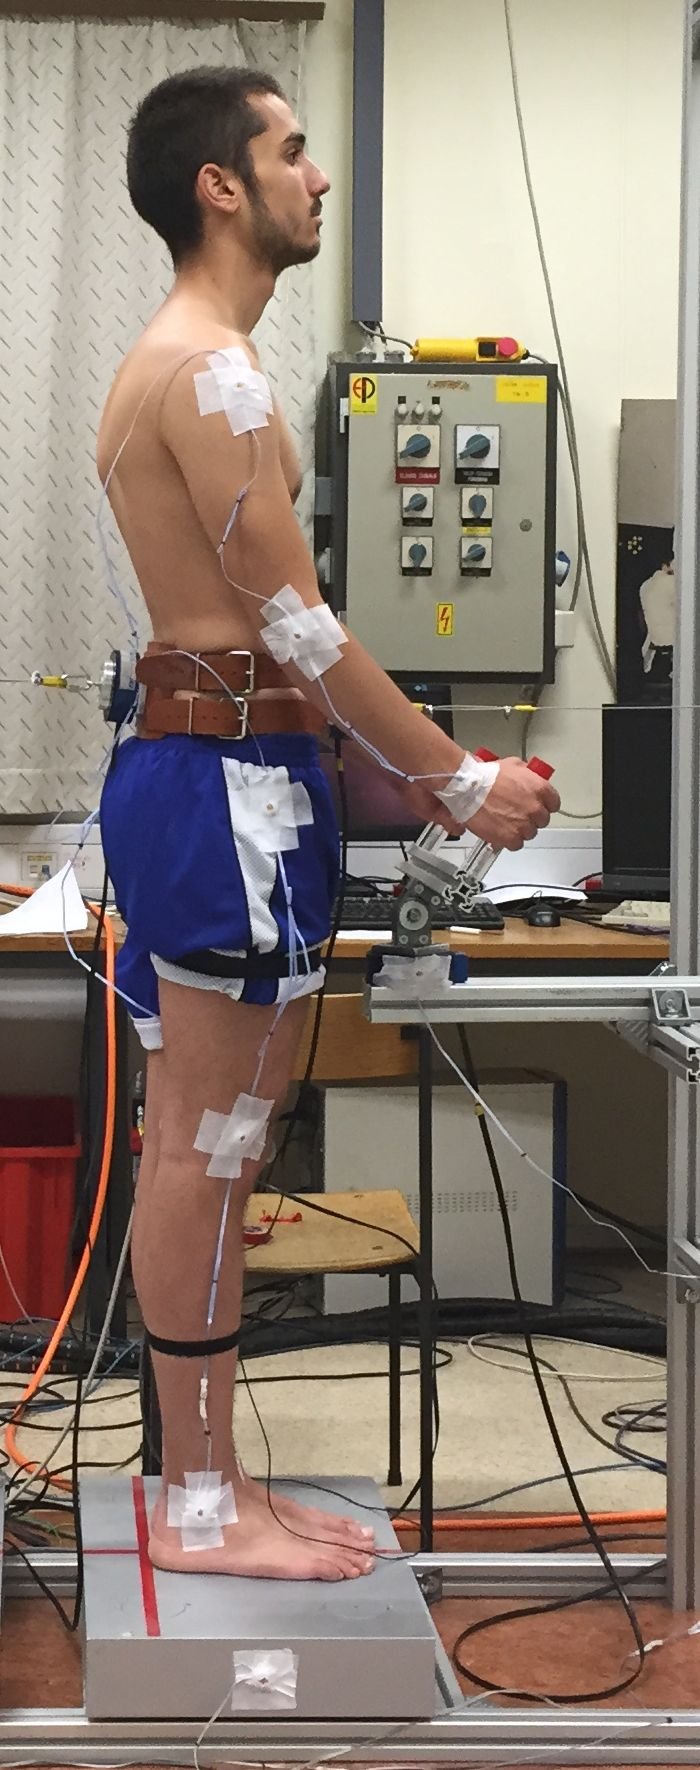
\includegraphics[width=0.2\columnwidth]{low.jpg} &
		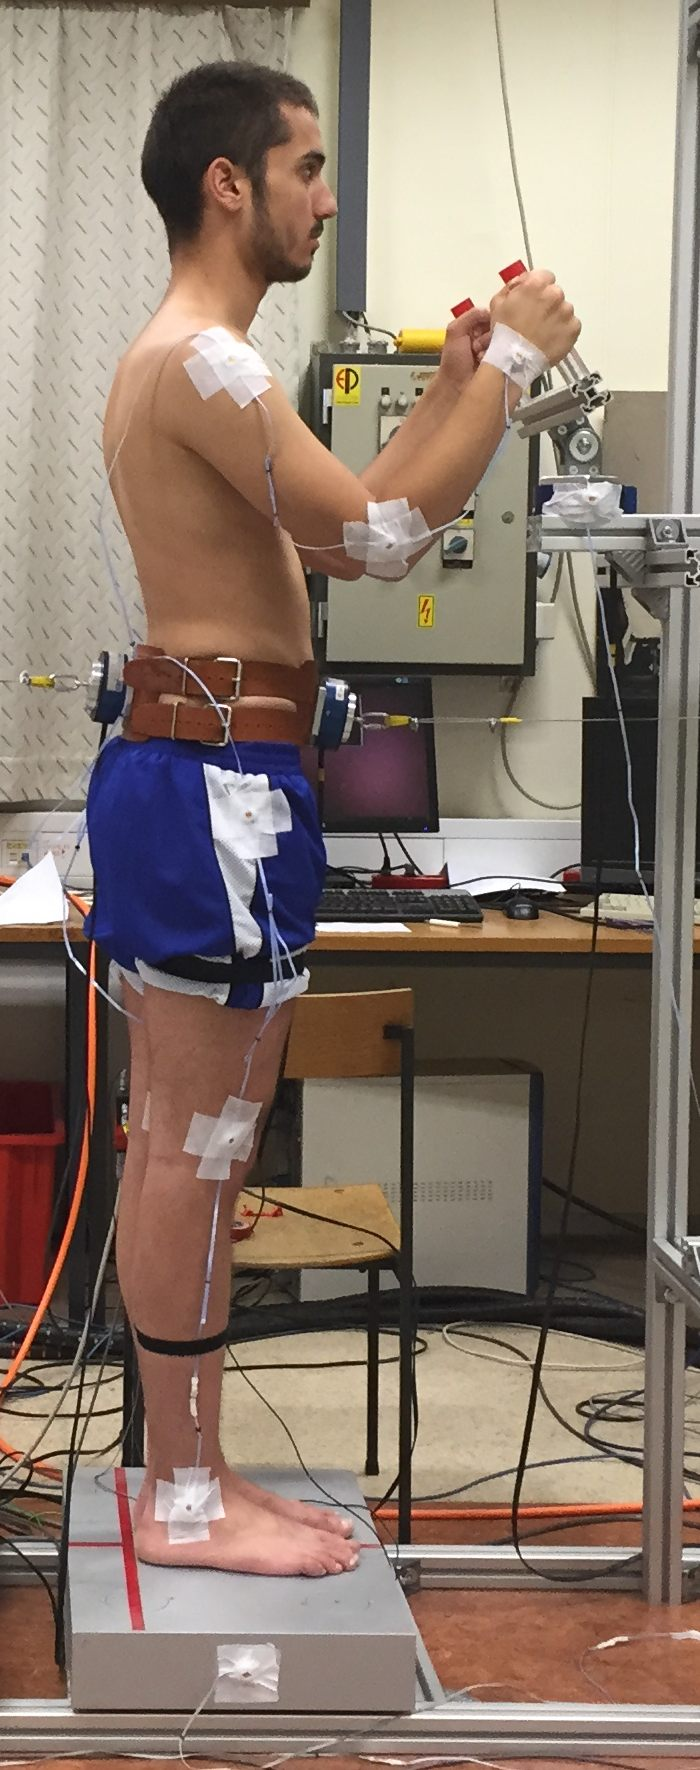
\includegraphics[width=0.2\columnwidth]{mid.jpg} &
		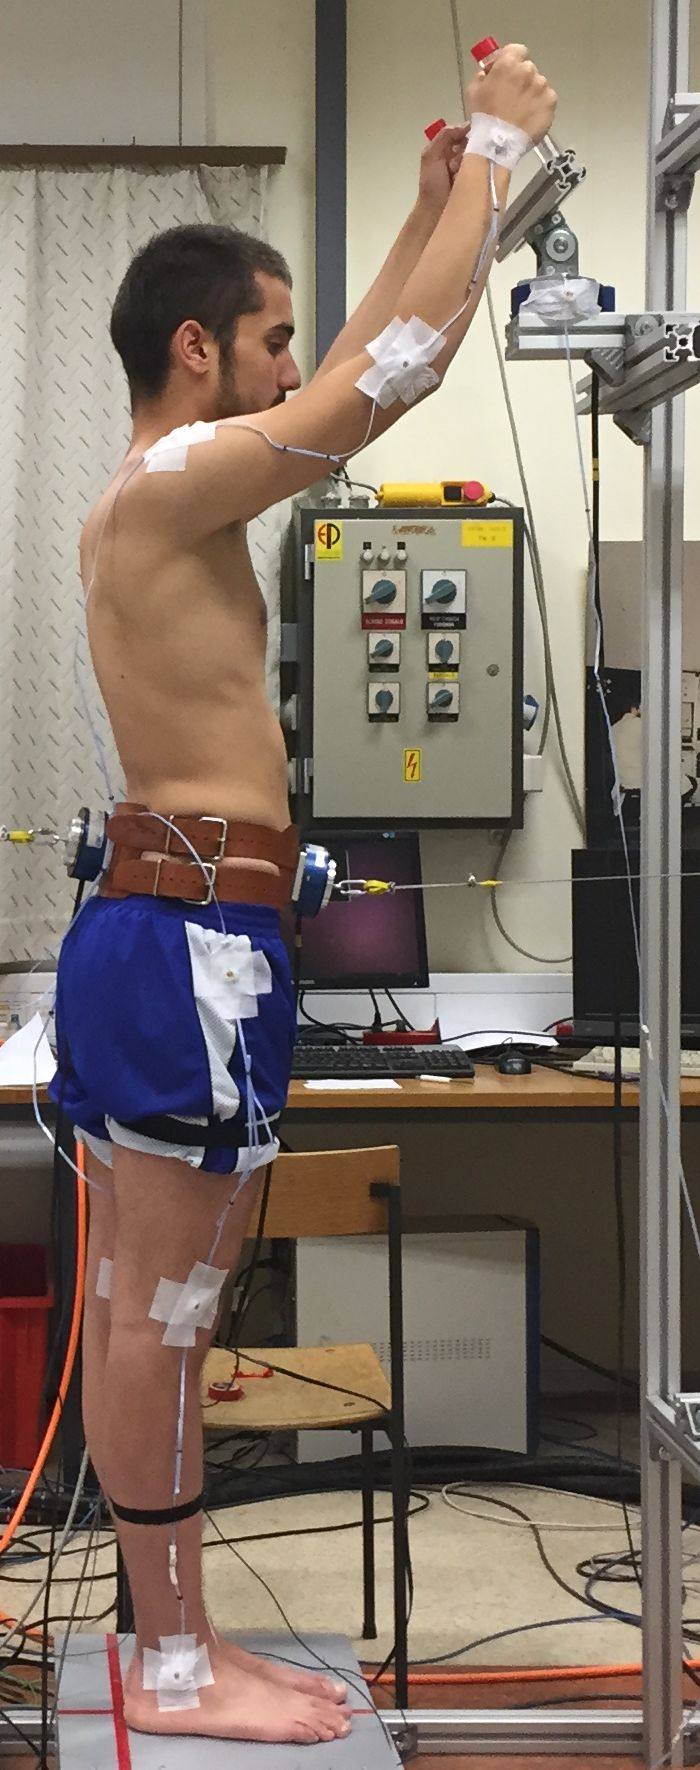
\includegraphics[width=0.2\columnwidth]{high.jpg} \\
		(b) & (c) & (d) & (e)
	\end{tabular}
	\caption{Experiments setup for five different positions: (a) stance, (b)
		wide stance, (c) low handle, (d) middle handle and (d) high handle.  A
		pulley mechanism, which is connected to the subject by a belt, perturbs
		the subject's CoM. Contact forces are measured at the feet and hands.
		Motion is recorded with an optical motion capture system.}
	\label{experimentsetup}
\end{figure}


\textbf{Methods:} Eleven healthy male subjects participated in this study.  Their average age
was $21.7$ years (SD $=2.2$ years), height = $183$ cm (SD $=4.6$ cm) and body
mass $76.8$ kg (SD $=8.1$ kg).  The subjects were informed about the course of
the study prior to their participation and were required to sign an informed
consent approved by the National Medical Ethics Committee (No. 112/06/13).

We observed the subject’s reactions to the external perturbations in five
different poses.  In the first pose (\textit{stance}), subjects were standing
straight with their feet together and arms crossed over the torso
(Fig.~\ref{experimentsetup}.a).  In the second pose (\textit{wide stance}),
subjects were standing with their arms crossed over the torso and their left
foot $60$ cm ahead of their right foot (ankle to ankle distance).  In the
third pose (\textit{low handle}), subjects were standing as in the first pose
and holding the handle which was located in front of their bodies at the hip
height (Fig.~\ref{experimentsetup}.b).  In the fourth pose (\textit{middle
	handle}), subjects were standing as in the first pose and holding the handle
which was located in front of their bodies at the shoulder height
(Fig.~\ref{experimentsetup}.c).  In the last pose (\textit{high handle}),
subjects were standing as in the first pose and holding the handle which was
located in front of their bodies and above the head
(Fig.~\ref{experimentsetup}.d).

The subjects were perturbed by a horizontal external force produced by our
force-controlled pulling mechanism \cite{Peternel&Babic13} at the approximate
position of their CoM \cite{Gardetal04}.  The command signal was a step with
$0.5$ second width (see Fig.~\ref{perturbations}).  The actual perturbation
force was controlled by a combination of a feed-forward and a PID feedback
controller.  We selected eight linearly increasing magnitudes of perturbation
forces where the maximum was defined as 22\% of the individual subject's body
weight and the minimum was $1/8$ of the maximum force (increasing rate of
$1/8$ of the maximum).  Between each perturbation we induced a random pause.
For each pose, we repeated the series of eight perturbations ten times (80
trials per subject per pose) and observed the human reactions.  We gave the
subjects 10 minutes pause between each pose.  In case of the first pose, the
subjects had to step before the maximum perturbation was reached.  When the
subject made a step, the experimenter stopped the procedure and moved to the
next series of perturbations.  The step was not required in other poses and
the series of perturbations repeated uninterrupted.
\begin{figure}
	\centering
	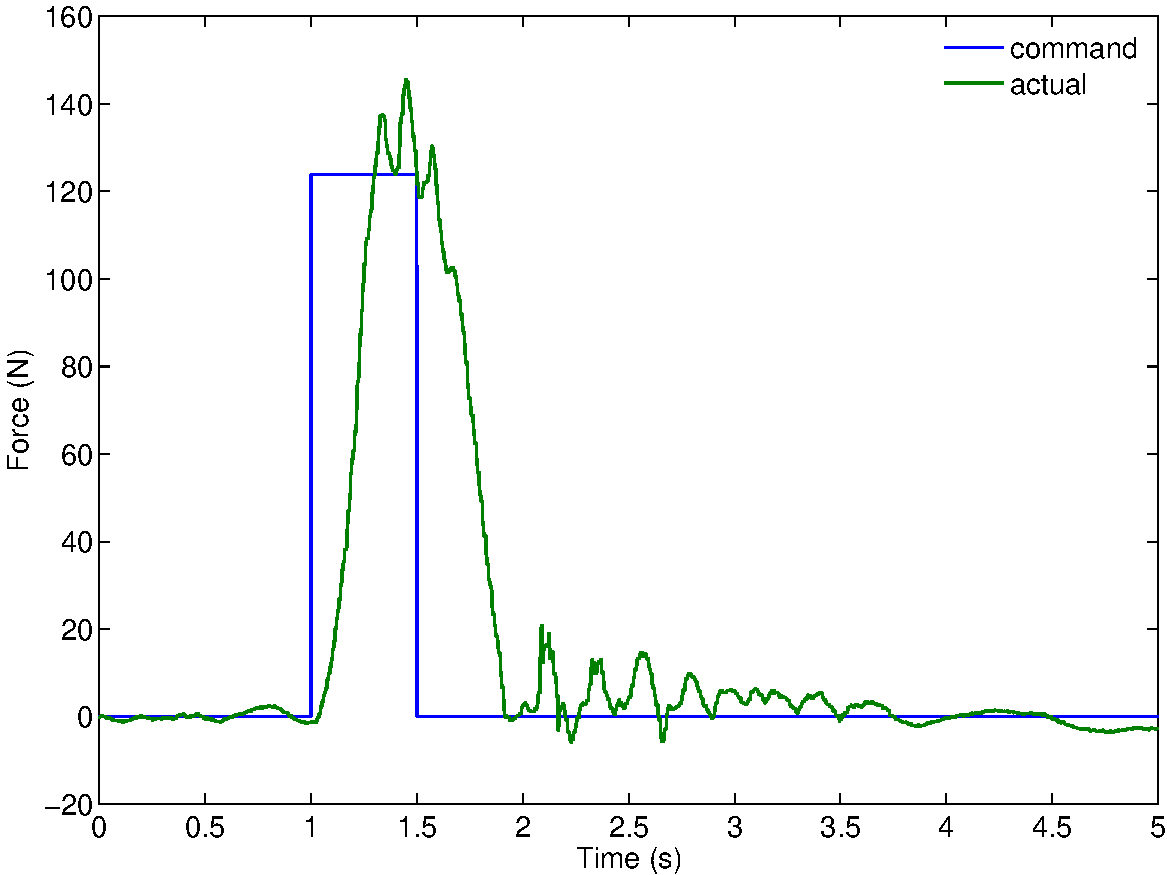
\includegraphics[scale=0.4]{perturbation.pdf}
	\caption{An example of the perturbation force applied to the CoM of the
		subjects.  This is for the subject whose body mass is $76.5$ kg.  The
		intensity of the perturbation is number $6$ meaning that the force is
		$6/8$ of the maximum for this subject.}
	\label{perturbations}
\end{figure}

Body movements were measured by a motion capture system (3D
Investigator$^{\tt\small TM}$ Motion Capture System, NDI, Waterloo, Ontario).
The optical markers were placed on the ankle, knee, hip, shoulder, elbow and
wrist.  The positions of the markers are used to calculate the joint angles.
We used two force plates (9281CA, Kistler Instrument AG, Winterthur,
Switzerland) to measure the ground reaction forces and center of pressure
position.  The handle was mounted on a 3-axis force sensor (45E15A, JR3,
Woodland, USA) to measure the force between the handle and the subject.

In order to estimate the starting time of the subjects' reactions, we measured
muscle activation in Triceps Brachii, Soleus and Tibialis Anterior by surface
electromyography (EMG).  We placed surface EMG electrodes (SX230 EMG sensor,
Biometrics Ltd, Newport, UK) on the selected muscles in accordance with SENIAM
recommendations \cite{Hermensetal99}.  We also placed a monitor in front of
the subject to provide visual feedback on the CoP position that allowed him to
move back to the initial pose after each perturbation.


\textbf{Model:} In the experiments, in order to produce movements which are planar only, we
prevented applying out-of-plane forces/moments to the subjects by providing a
pair of handles for them and perturbing them in a plane.  Therefore, we could
use planar models for both inverse dynamics and CoM manipulability
calculations.  Although, using a planar model for wide stance pose is a bit
unrealistic.  Planar humanoid models that we used for the stance, wide stance
and all three handle poses are shown in Fig.~\ref{planarhumanoids}.  These
models consist of multiple links which are connected to each other by actuated
revolute joints.  Note that lower legs are connected to the ground.  This is
because we assume that the feet of the subjects do not move during the
experiments.  To model the stance pose, we lock the DoF of the arms.  So, in
this case, the model has 3 DoF and is unconstrained.  For the wide stance, the
robot has 6 DoF and is constrained due to the kinematic loop in the legs.  For
the handle poses, the robot has five actuated DoF and it is constrained at the
hand to model the handle contact.
\begin{figure}
	\centering 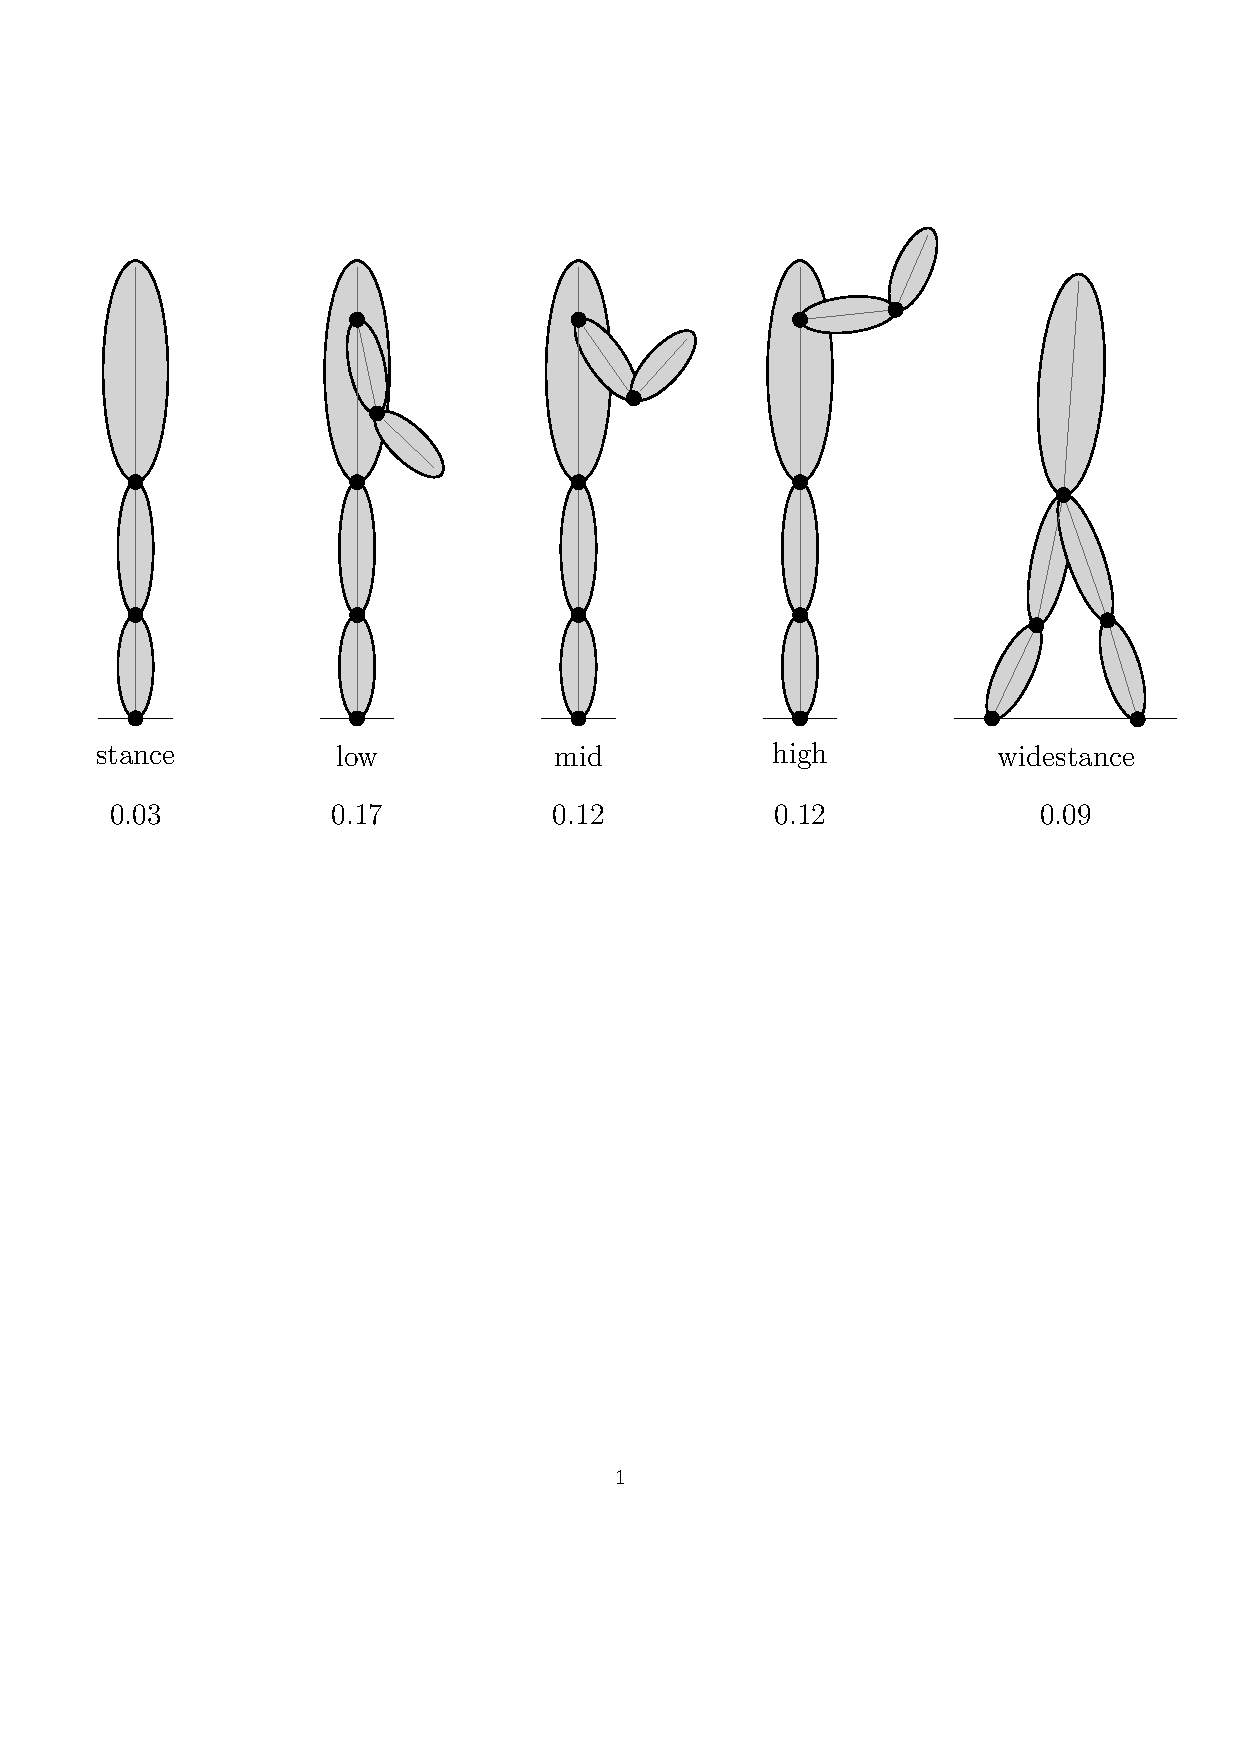
\includegraphics[trim = 13mm 154mm 10mm 37mm, clip,
	scale=0.85]{robotmodels}
	\caption{Schematic diagram of the planar humanoid robot model}
	\label{planarhumanoids}
\end{figure}

Since for balancing we are only interested in movements in the horizontal
direction, we calculated the maximum value of $\Delta \dot{\Bc}$ in this
direction for all five positions.  This represents the maximum achievable
change of velocity of the CoM in the horizontal direction and is a measure for
the ability to accelerate the CoM in order to correct its position in this
direction. Joint angles of the arms for the handle positions are
set to the average initial joint angles of the subjects that we calculate from
the marker positions.  For the low handle, the shoulder angle (angle between
torso and upper arm) is $12^\circ$ and the elbow angle (between upper and
lower arms) is $145^\circ$.  Shoulder and elbow angles are $35^\circ$ and
$77^\circ$ for the middle handle, and $96^\circ$ and $118^\circ$ for the high
handle positions, respectively.  For the wide stance position, we assume zero
angles in the knees and upright torso.  The weighting matrix that we use for
the calculations is a diagonal matrix as
%
\begin{equation}
\BW = diag([2.33, 3.45, 4.55, 1, 1.25]) \, ,
\end{equation}
%
which is determined to include the differences in the joint's strengths
\cite{Anderson2007, Bober2002, Gandevia1998, Moraux2013}.

Calculated values for the maximum $\Delta \dot{\Bc}$ for the five positions
are mentioned in Fig.~\ref{planarhumanoids}.  As it can be seen in this
figure, the low position has the highest value (i.e. $0.17$) for the
manipulability and the stance position has the lowest one (i.e. $0.03$).
Manipulability for the middle and high positions are the same ($0.12$) and
lower than the low position.  Also wide stance manipulability (i.e. $0.09$) is
only better than the stance position.  Therefore, according to the
manipulability analysis for our models, we expect the same ranking for the
five positions in the sense of total average required torque to keep the
balance.  We will verify this hypothesis in the next subsection.


\textbf{Results:} As already mentioned, inverse dynamics are used to compute the torques that
are applied (at the joints) by the human subjects.  Joint angles are
calculated by using marker positions, and joint velocities and accelerations
are estimated by using simple time differentiation.  Lengths and inertial
parameters of the subjects are calculated via the software that is introduced
in \cite{Zlajpah&Babic14}.  Feather stone's Spatial software package
\cite{Featherstone} is used for the dynamics calculations.

To work out the average total torque for each position and each perturbation
intensity, first we calculate the joint torques from inverse dynamics for each
trial (in total $4400$ trials $= 5$ poses $\times 8$ intensities $\times 10$
reps $\times 11$ subjects).  Then we calculate the average torque over the
reps for each joint.  Note that, since maximum achievable torque of the arm
joints vary with arm configuration, we normalize shoulder and elbow torques
for the handle positions \cite{Anderson2007, Bober2002, Gandevia1998,
	Moraux2013}.  Then, we sum up the normalized joint torques to get $440$
(i.e. $5$ poses $\times 8$ intensities $\times 11$ subjects) values for the
average normalized joint torques.  The beginning time is the subjects' average
initial reaction time which is estimated by the average EMG signal.  The end
time is roughly the time that the subjects have recovered from the
perturbations.

%The same process gives us the average joint works.  The work is in fact the
%sum of $|\Btau \dot{\Bq}| \Delta t$, where $\Delta t$ is the data gathering
%frequency which is 2 milliseconds in our experiments.  We take the sum from
%$t=1.2$ s to $t=3$ s.

%% The values of the calculated normalized joint torques for the five positions
%% and different perturbation intensities are shown in
%% Fig.~\ref{jointtorquesubjects} for all subjects.  These values are marked by
%% $+$ In The graphs.  The Lines in the graphs are fitted to the values by using
%% least squares method.  Note that the graph of the first subject does not
%% include the results for high handle position.  This is due to the problem in
%% data gathering during the experiment which is solved for the next subjects.
%% \begin{figure}
%%   \centering
%%   \begin{tabular}{cc}
%%     subject 1 & subject 2 \\
%%     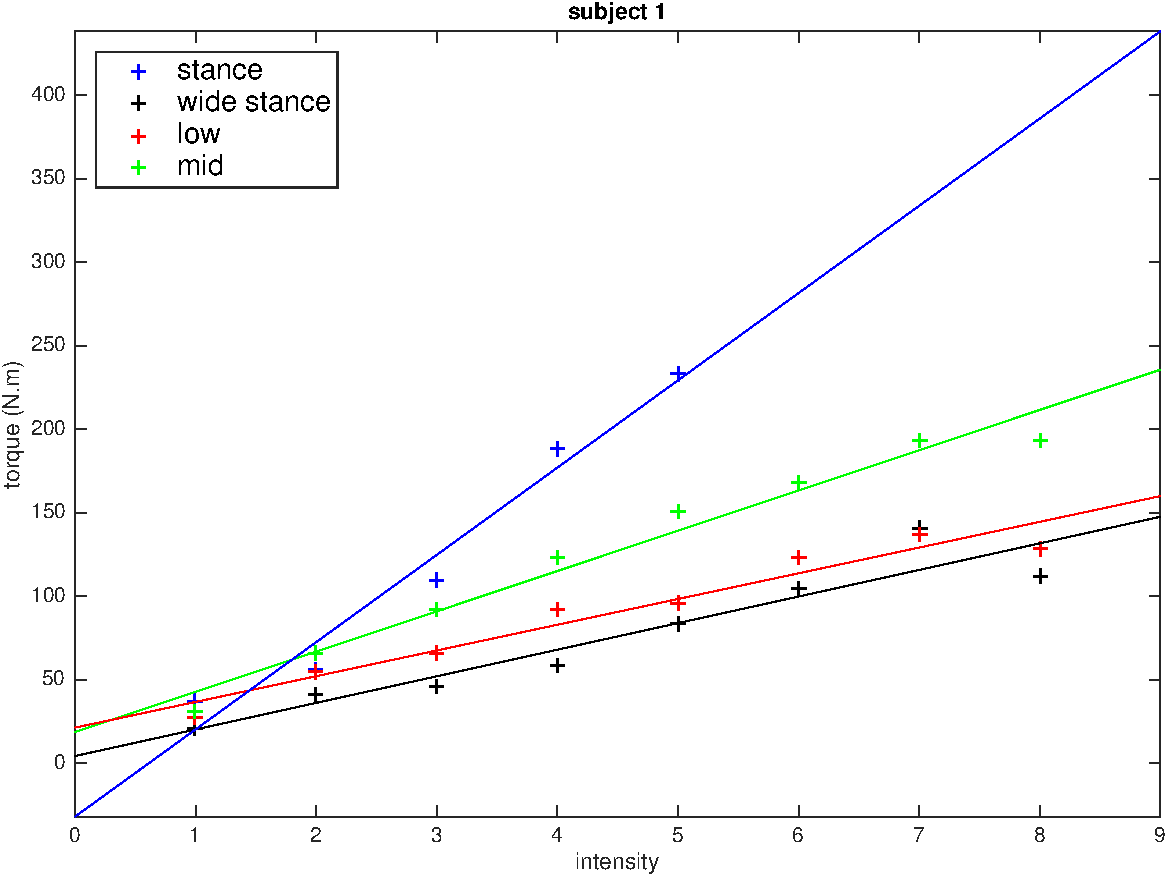
\includegraphics[width=0.46\linewidth]{subj1} &
%%     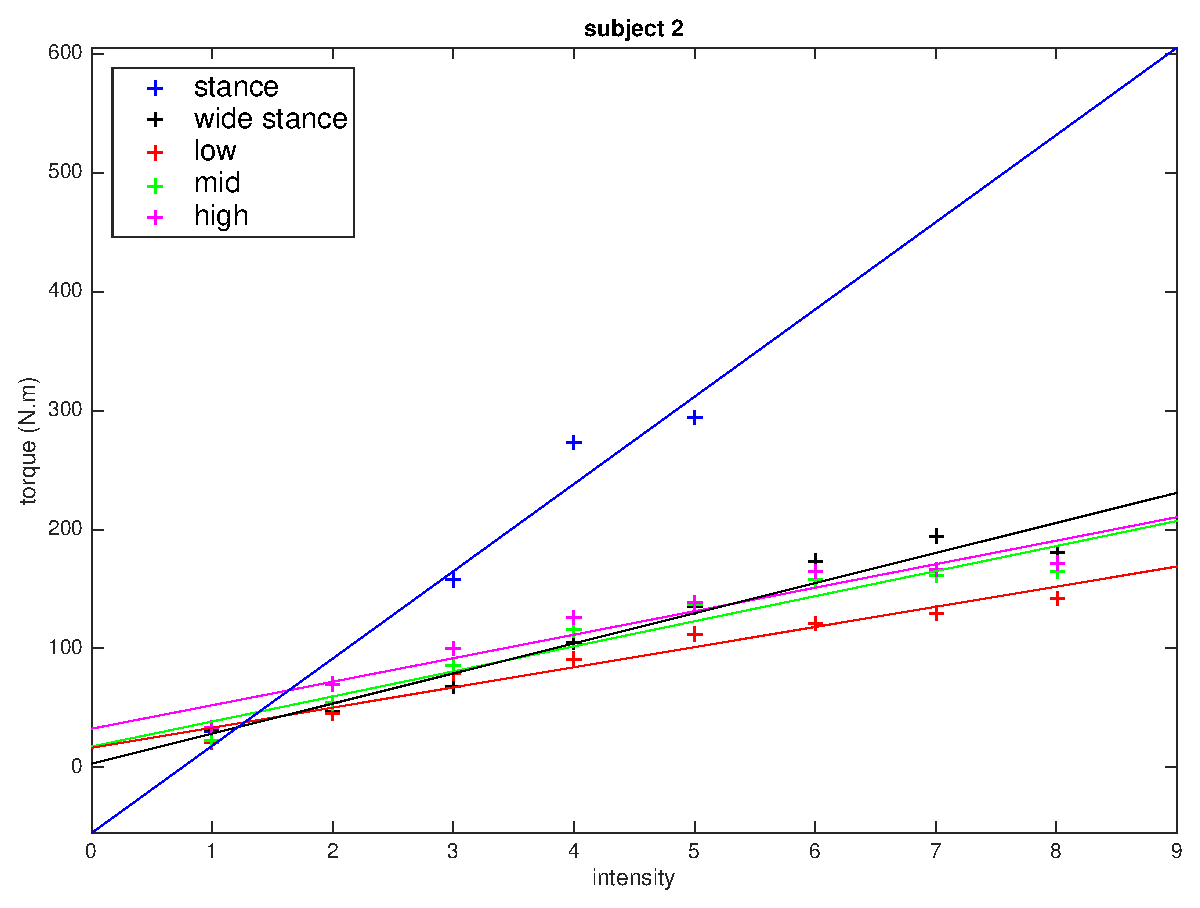
\includegraphics[width=0.46\linewidth]{subj2} \\
%%     subject 3 & subject 4 \\
%%     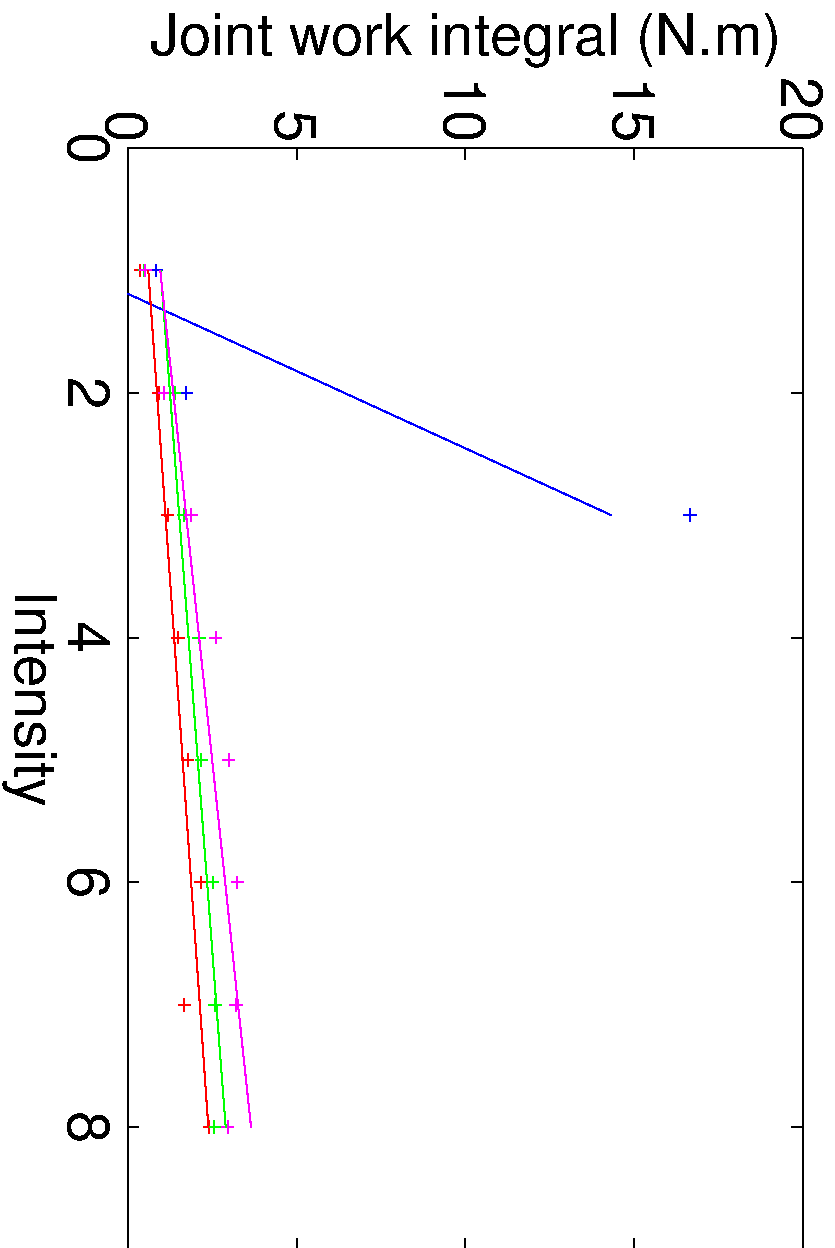
\includegraphics[width=0.46\linewidth]{subj3} &
%%     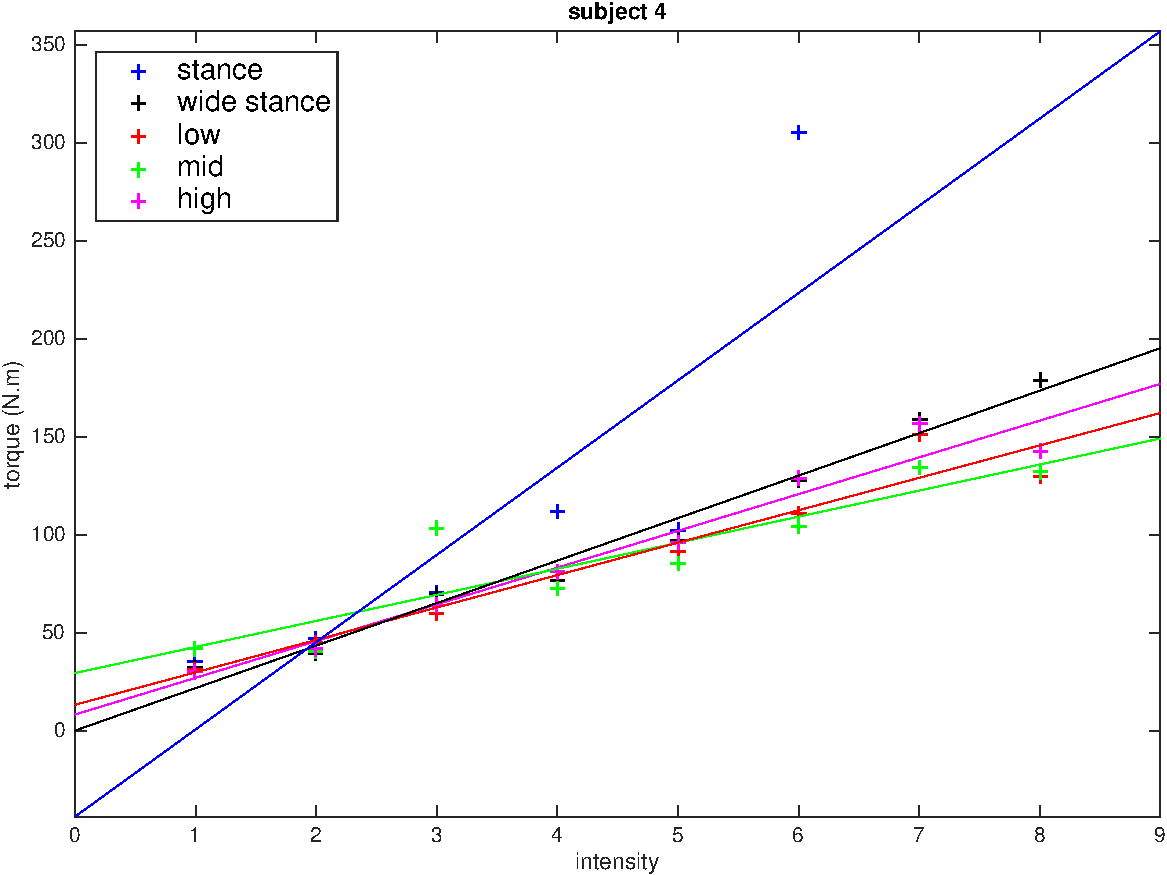
\includegraphics[width=0.46\linewidth]{subj4} \\
%%     subject 5 & subject 6 \\
%%     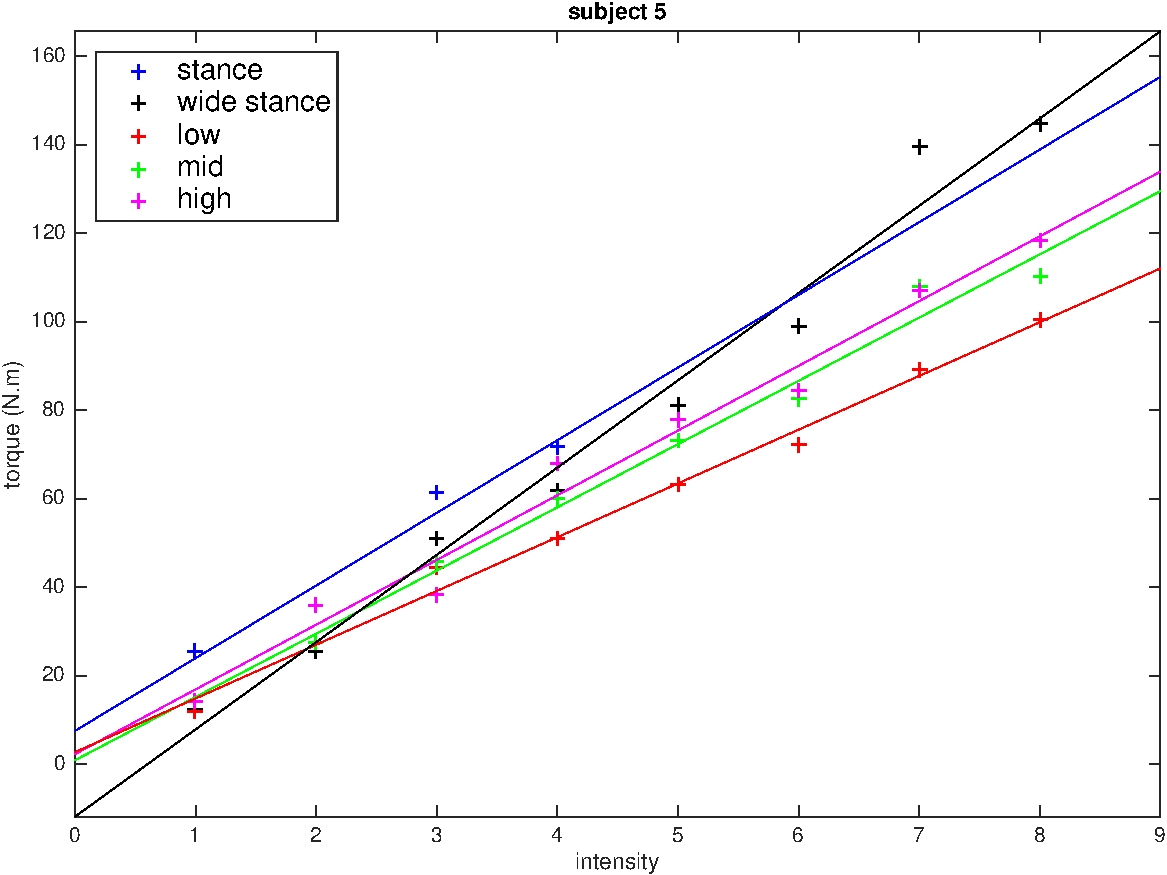
\includegraphics[width=0.46\linewidth]{subj5} &
%%     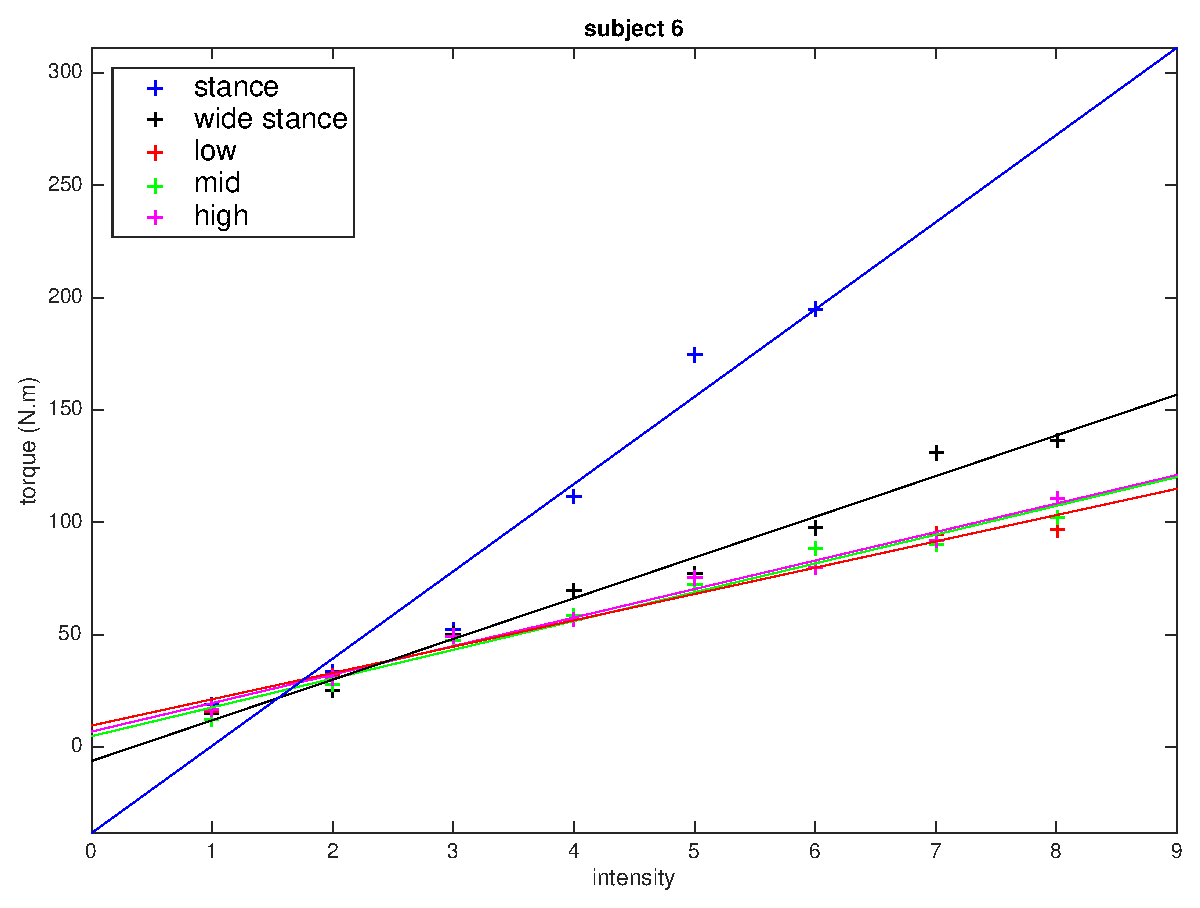
\includegraphics[width=0.46\linewidth]{subj6} \\
%%     subject 7 & subject 8 \\
%%     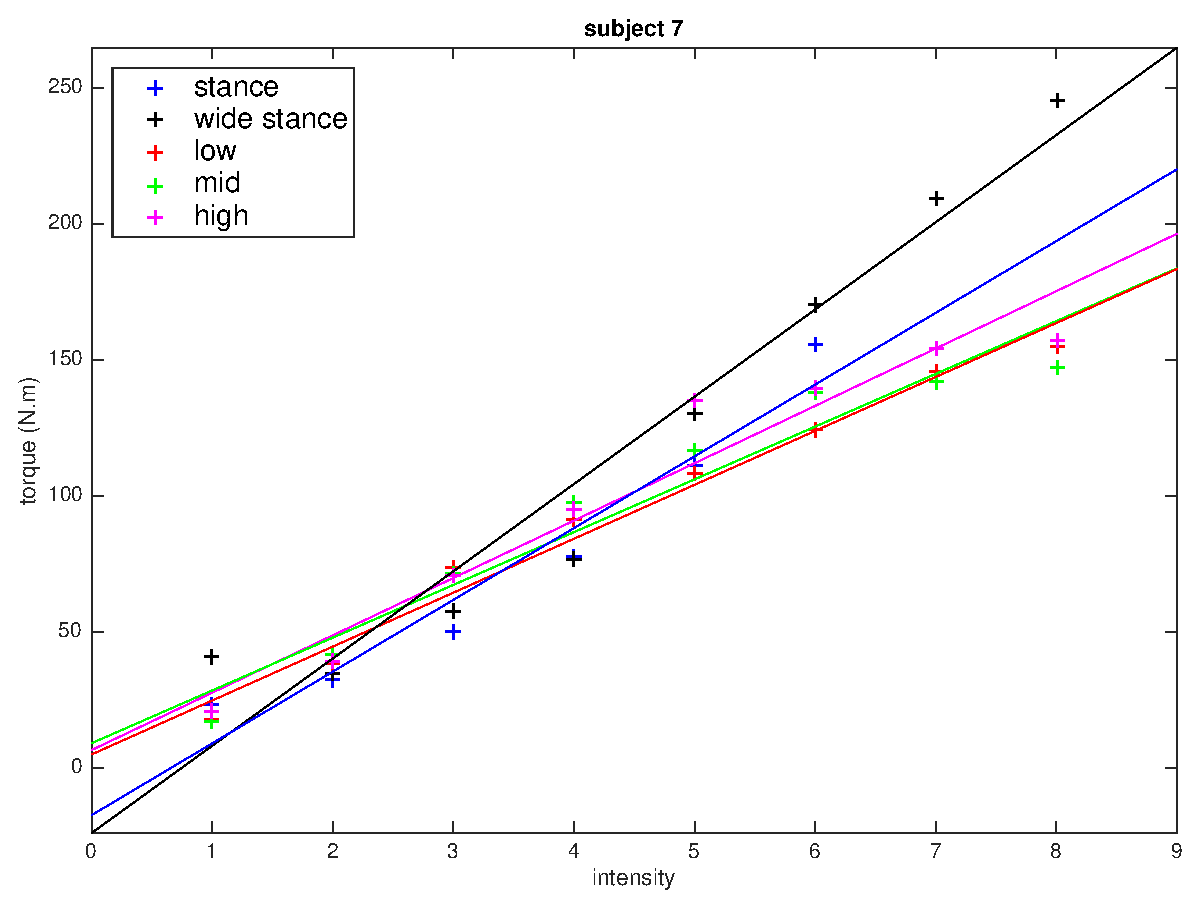
\includegraphics[width=0.46\linewidth]{subj7} &
%%     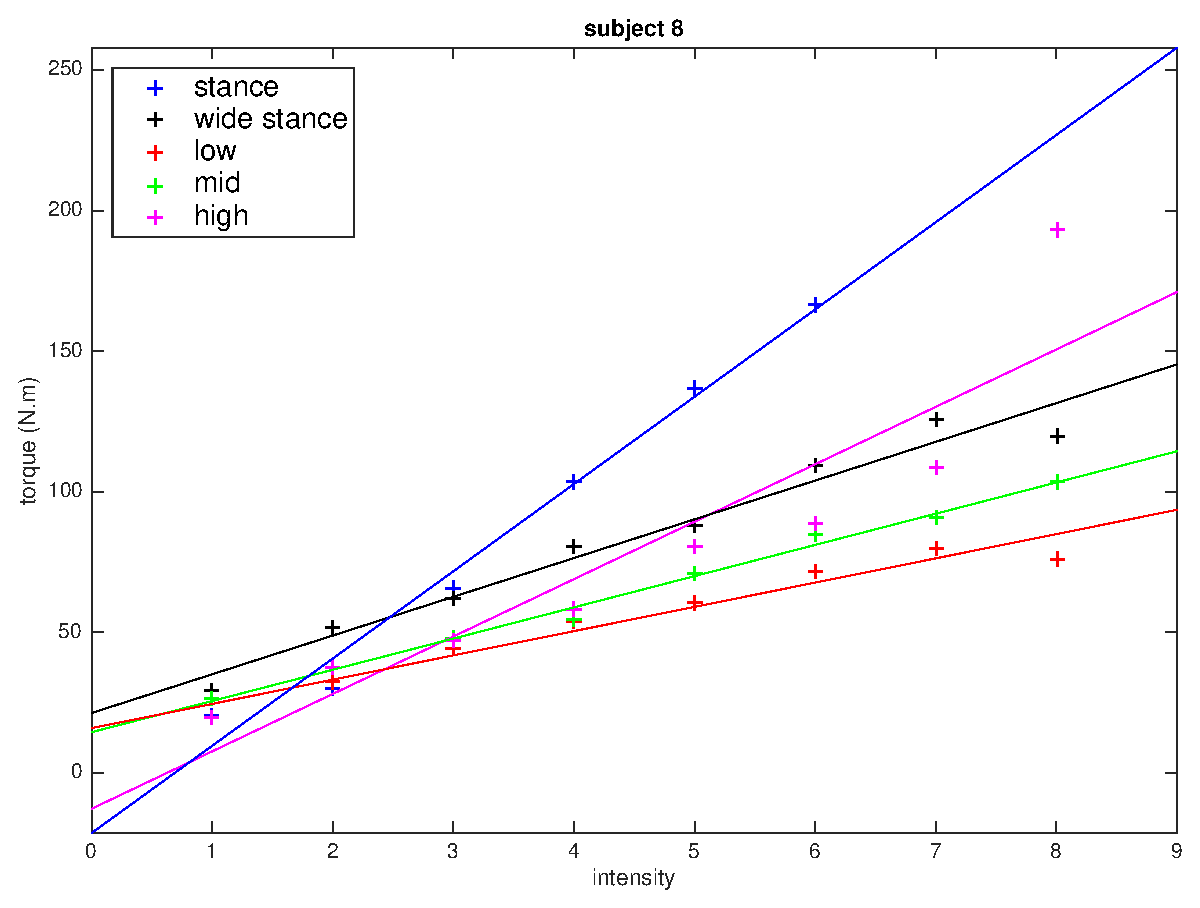
\includegraphics[width=0.46\linewidth]{subj8} \\
%%     subject 9 & subject 10 \\
%%     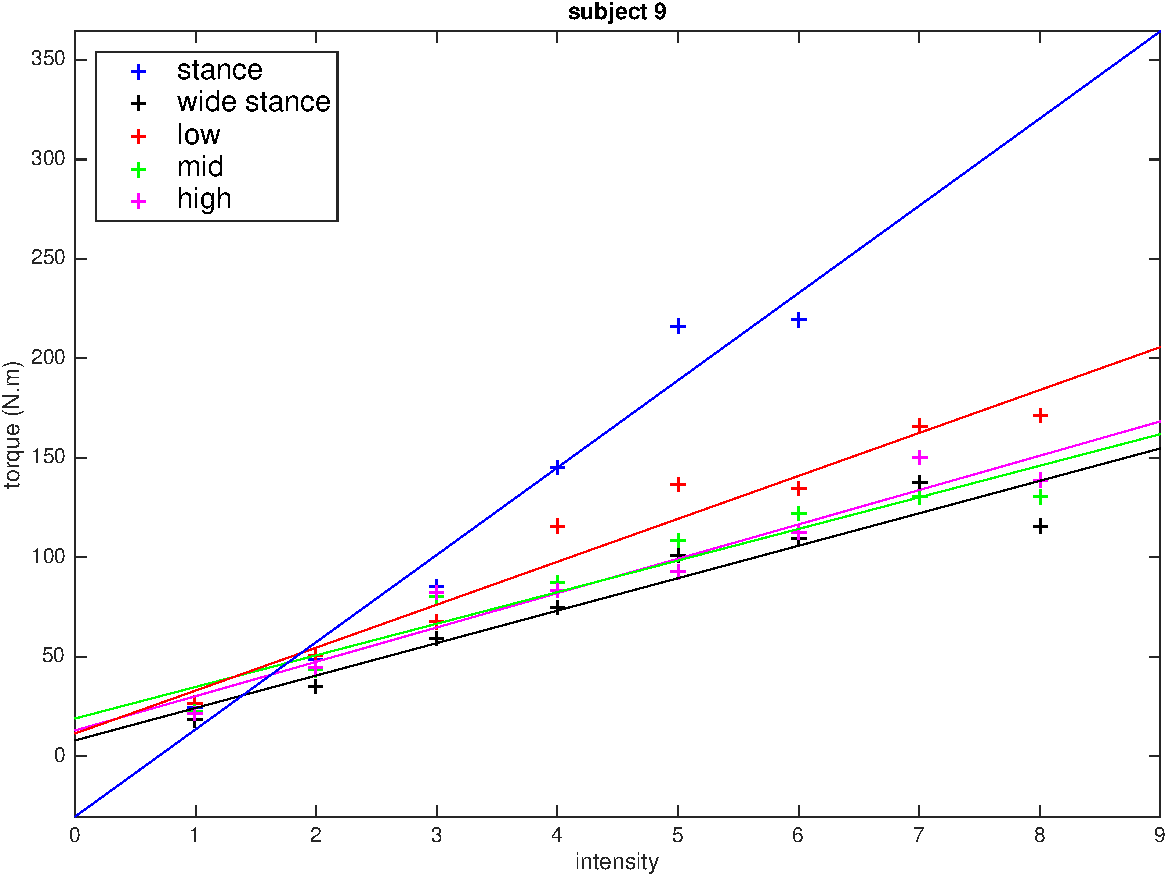
\includegraphics[width=0.46\linewidth]{subj9} &
%%     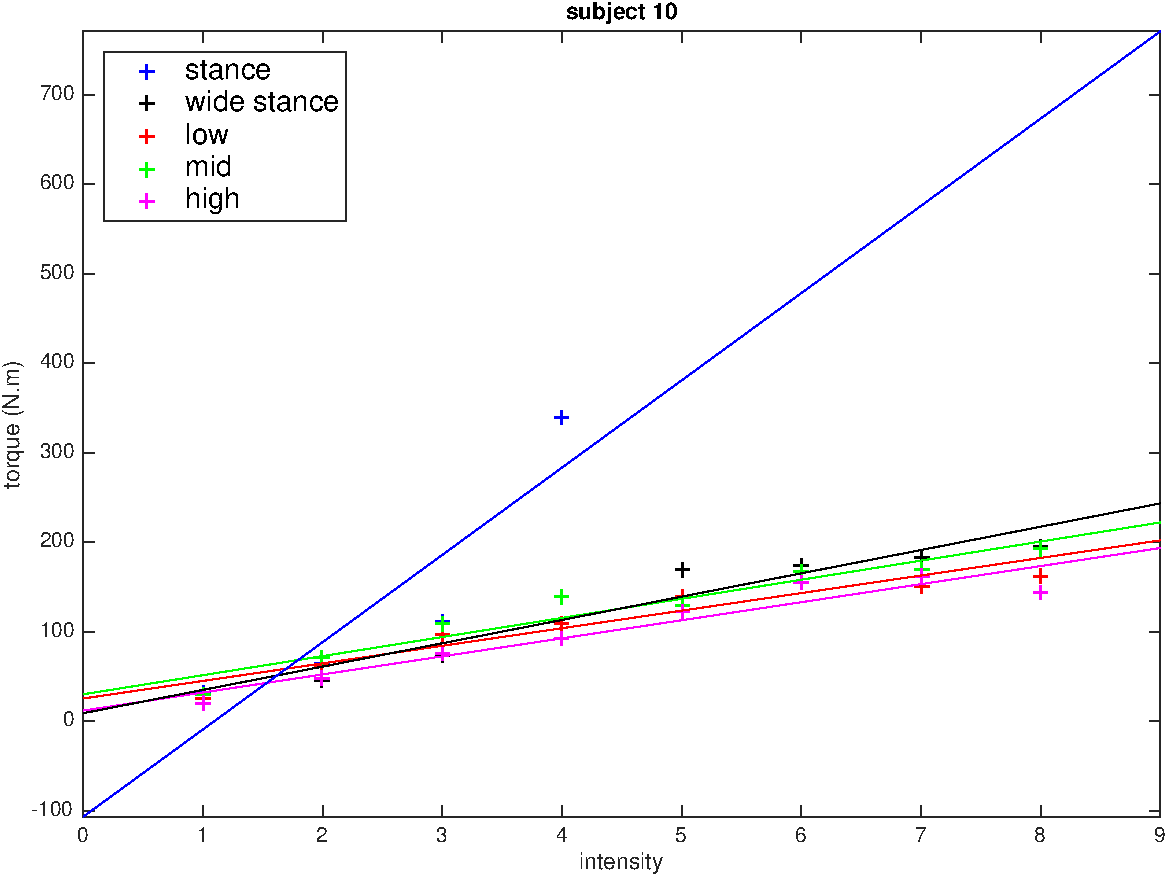
\includegraphics[width=0.46\linewidth]{subj10} \\
%%   \end{tabular}
%%   \caption{Total average normalized joint torques for the subjects at
%%     different perturbation magnitudes and different poses: stance (blue), low
%%     handle (red), middle handle (green) and high handle (magenta).}
%%   \label{jointtorquesubjects}
%% \end{figure}

The means of the normalized joint torques (per subjects) is shown in
Fig.~\ref{jointtorque}.  This figure shows the total average torque (after
removing outliers) for all subjects at each configuration and each intensity.
The lines are fitted to the values by using least squares method.  The
standard error of the means are also shown in this figure.  As can be seen in
this figure, the low handle pose has the lowest total torque and the stance
pose has the highest.  According to this graph, the ranking between the
positions is 1) low, 2) middle, 3) high, 4) wide stance and 5) stance.  This
ranking is more visible in higher intensities and it conforms with the
manipulability numbers from our analysis.  The only difference is that
manipulability analysis predicts that middle and high positions are the same
whereas experimental results show a bit difference between two (middle is
better than high).  Therefore, the experimental results agree with the
manipulability analysis in the previous subsection.  Configurations of greater
manipulability require less torque, in order to maintain balance after
perturbations of equivalent magnitudes.
\begin{figure}
	\centering 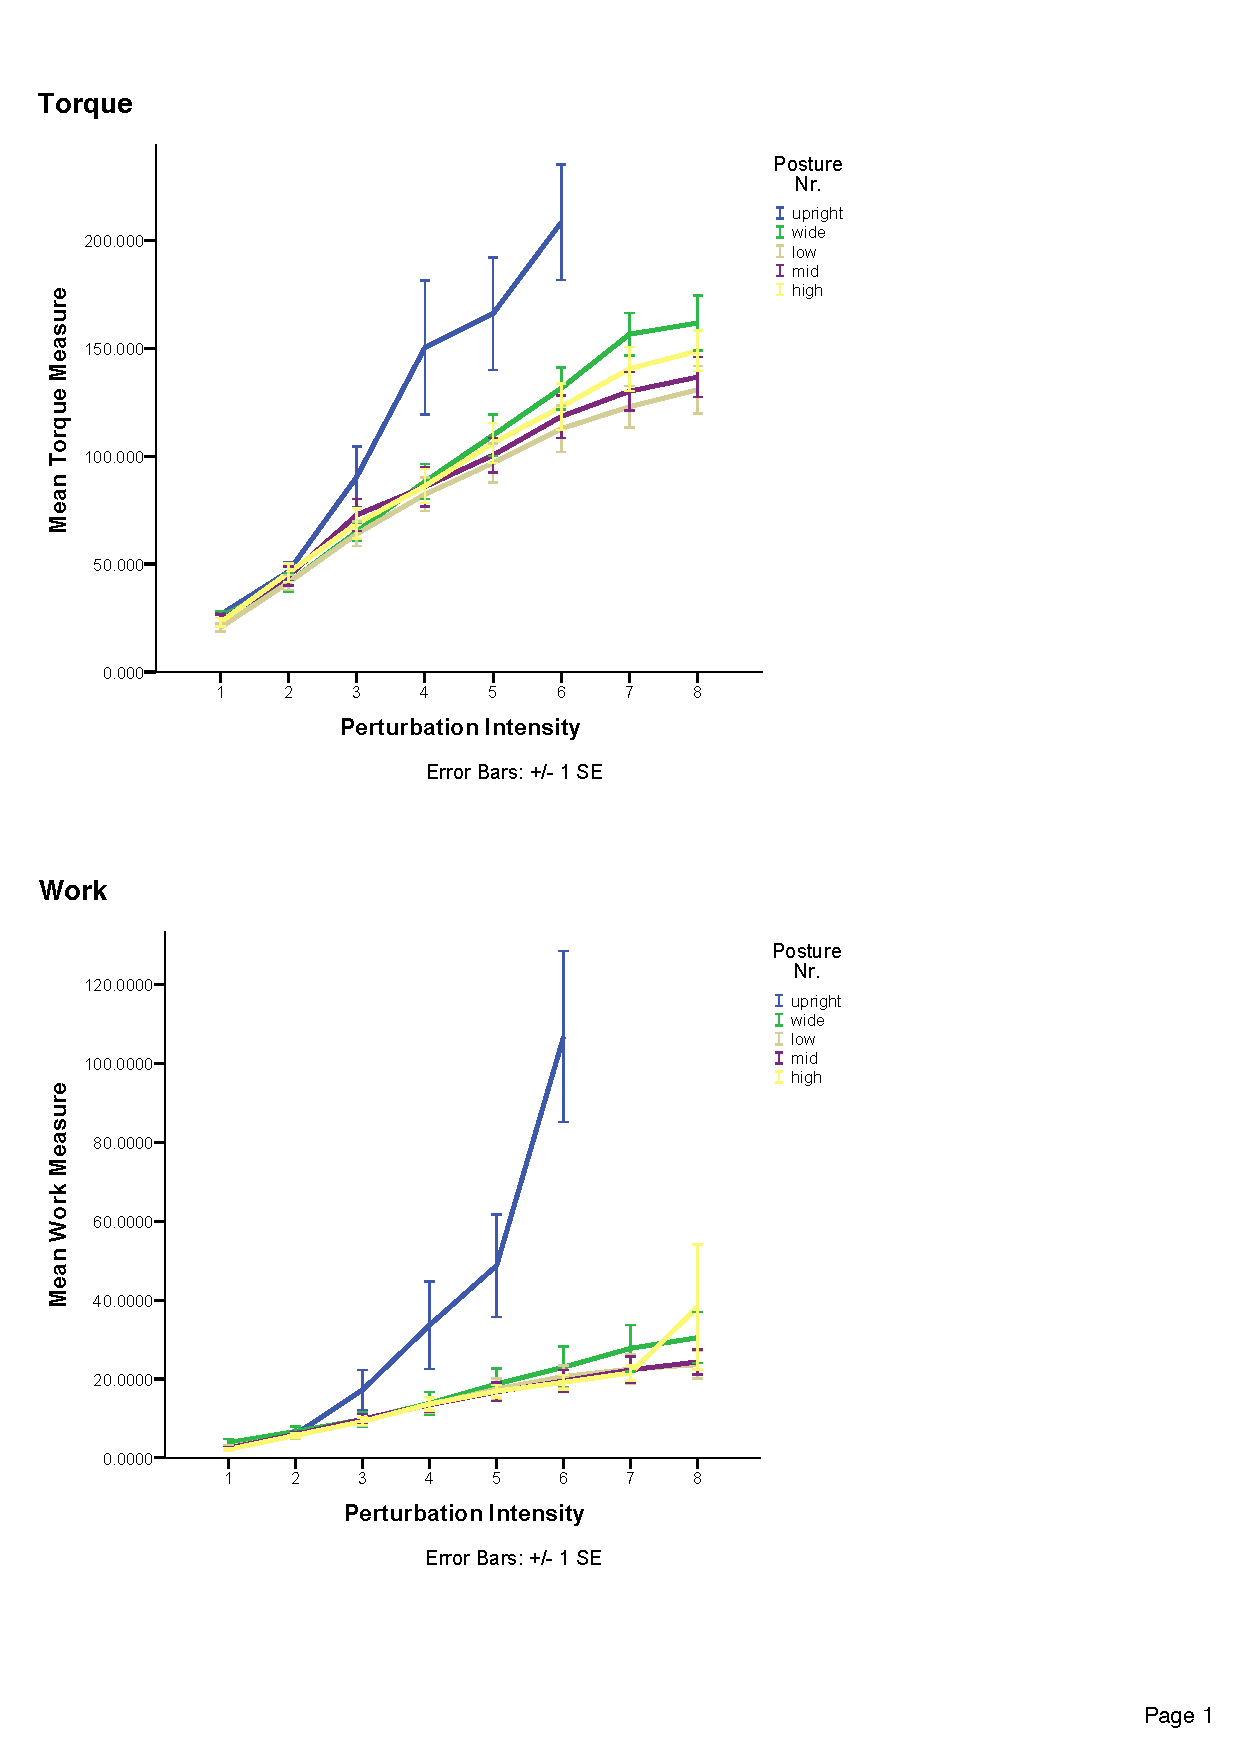
\includegraphics[trim = 1mm 150mm 10mm 10mm, clip, scale =
	0.95]{errorBarPlotsSEM-norm_v2}
	\caption{Average of the total torque for the subjects at each pose and each
		perturbation intensity.  The stance position required the most torque in
		order to maintain balance.  While the low handle position required the
		least amount of torque for the same perturbation.}
	\label{jointtorque}
\end{figure}


\textbf{Conclusion:} A set of metrics are introduced in this chapter to study, analyse and measure
the ability to balance for humans and robots.  These metrics, which are called
the manipulability of the center of mass, provide two types of ellipsoids
which graphically show how the CoM can be accelerated in 3D space by a certain
amount of change of motion (due to impulses) at the joint space.  These
ellipsoids can be used to measure torque efficiency and maneuverability of
humans and robots.  The proposed metrics are applicable to floating base
robots with non-breakable contacts with the environment.  Also, experiments on
human subjects are performed to investigate the applicability of the proposed
metrics for human studies.  In the experiments, the standing subjects (in five
different configurations) were perturbed by a controlled force acting on their
CoM.  Then, the selected configurations were ranked according to the average
total torque that is applied by the subjects to recover their balance at each
configuration.  It is shown that the proposed metric for torque efficiency can
successfully predict the same ranking between the configurations as the
experimental results suggested.  This agreement shows the applicability of the
metrics for human studies as well.  Therefore, manipulability of the center of
mass provides greater insight into the posture controllability of humans and
robots, in various configurations and contact conditions.